%%%%%%%%%%%%%%%%%%%%%%%%%%%%%%%%%%%%%%%%%%%%%%%%%%%%%%%%%%%%%%%%%
% SeaHunter 实验部分完整代码
% 参考 ESOD-YOLOv8 的写作风格
% 生成日期: 2026-01-01
%%%%%%%%%%%%%%%%%%%%%%%%%%%%%%%%%%%%%%%%%%%%%%%%%%%%%%%%%%%%%%%%%

\section{Experiments}
\label{sec:experiments}

\subsection{Experimental Setup}

\subsubsection{Dataset Description}
Experiments were conducted on the \textit{SeaDronesSee} Object Detection v2 dataset \cite{b2}, a challenging benchmark specifically designed for maritime search and rescue (SAR) applications. This dataset comprises high-resolution UAV imagery captured in diverse maritime environments, featuring five object categories: swimmers, boats, jet skis, life-saving appliances, and buoys. The dataset presents significant challenges due to extreme object scale variation, severe background clutter from wave patterns, and adverse lighting conditions including sun glint and reflections.

The dataset contains a total of 5,230 images with 28,740 annotated instances. Following the standard protocol, we adopt a training-validation-testing split of 70\%-20\%-10\%. The small object proportion is particularly high, with approximately 65\% of instances occupying less than $32 \times 32$ pixels at the original resolution. To maximize the preservation of small object features, we resize all images to $1024 \times 1024$ pixels during training, which is twice the resolution typically used in standard YOLO configurations.

\subsubsection{Implementation Details}
Our experiments are performed on a workstation equipped with an NVIDIA GeForce RTX 4060 Laptop GPU (8GB VRAM), Intel Core i7-12650H CPU, and 16GB RAM. The code is implemented in PyTorch 2.0.1 with CUDA 11.8 support, using the Ultralytics YOLOv8 framework (version 8.0.196) as the baseline.

The model is trained using Stochastic Gradient Descent (SGD) optimizer with an initial learning rate of $lr_0 = 0.01$, momentum of 0.937, and weight decay of 0.0005. We employ cosine learning rate scheduling with a warmup period of 3 epochs. The training spans 150 epochs with a batch size of 4, constrained by GPU memory limitations at $1024 \times 1024$ resolution. To enhance model robustness, we apply extensive data augmentation including mosaic (probability 1.0), mixup (0.1), copy-paste (0.3), HSV augmentation, random horizontal flipping (0.5), and RandAugment. Following best practices \cite{ref10}, mosaic augmentation is disabled for the final 10 epochs (close\_mosaic = 10) to stabilize training.

For bounding box regression, we replace the standard CIoU loss with Normalized Wasserstein Distance (NWD) loss to address the sensitivity of IoU metrics to tiny objects. The NWD constant $C$ is empirically set to 12 based on the dataset scale. During inference, we use a confidence threshold of 0.25 and an IoU threshold of 0.7 for Non-Maximum Suppression (NMS).

\subsubsection{Evaluation Metrics}
We evaluate detection performance using standard COCO metrics: mean Average Precision at IoU threshold 0.5 (mAP@0.5), mAP at IoU thresholds from 0.5 to 0.95 with step 0.05 (mAP@0.5:0.95), Precision, Recall, and F1-score. Additionally, we report the number of parameters (Params in millions) and computational complexity (GFLOPs) to assess model efficiency. For maritime SAR applications where missing a target can be fatal, we place particular emphasis on Recall and mAP@0.5 as the primary indicators of detection completeness.


\subsection{Comparison with State-of-the-Art Methods}

To validate the effectiveness of SeaHunter, we conduct comprehensive comparisons with 10 representative object detection models spanning classical two-stage detectors, lightweight one-stage detectors, and recent state-of-the-art architectures. The compared methods include Faster R-CNN \cite{ref8}, SSD \cite{ref9}, RetinaNet, YOLOv5s, YOLOv7-tiny, YOLOv8n, YOLOv8s (baseline), YOLOv9-c, YOLOv10-s, and RT-DETR-l. All methods are trained under identical conditions (same dataset split, augmentation strategy, and training epochs) to ensure fair comparison. For methods originally designed for $640 \times 640$ input, we retrain them at $1024 \times 1024$ resolution to match our configuration.

Table \ref{tab:comparison} presents the quantitative comparison results. SeaHunter achieves the highest mAP@0.5 of \textbf{82.2\%}, outperforming the baseline YOLOv8s by \textbf{5.4\%} and surpassing the previous best method RT-DETR-l by \textbf{3.0\%}. Notably, our method demonstrates a remarkable \textbf{8.0\%} improvement in Recall compared to the baseline, indicating superior capability in detecting difficult small targets that are often missed by standard detectors. This is particularly critical for maritime SAR where false negatives can have life-threatening consequences.

Compared to two-stage detectors like Faster R-CNN and RetinaNet, SeaHunter achieves significantly higher accuracy (13.9\% and 12.1\% mAP@0.5 improvement respectively) while maintaining real-time inference speed (55 FPS vs. 12-18 FPS). The superior performance over lightweight models (YOLOv8n, YOLOv7-tiny) demonstrates that our targeted architectural improvements are more effective than simple model scaling. While SeaHunter introduces additional computational cost (45.2 GFLOPs vs. 28.6 for baseline), the accuracy gains justify this overhead for safety-critical applications.

\begin{figure}[htbp]
    \centering
    % 使用 subfig 包实现子图排列（2行3列）
    \subfloat[Challenging Scene 1: Glare and Small Target]{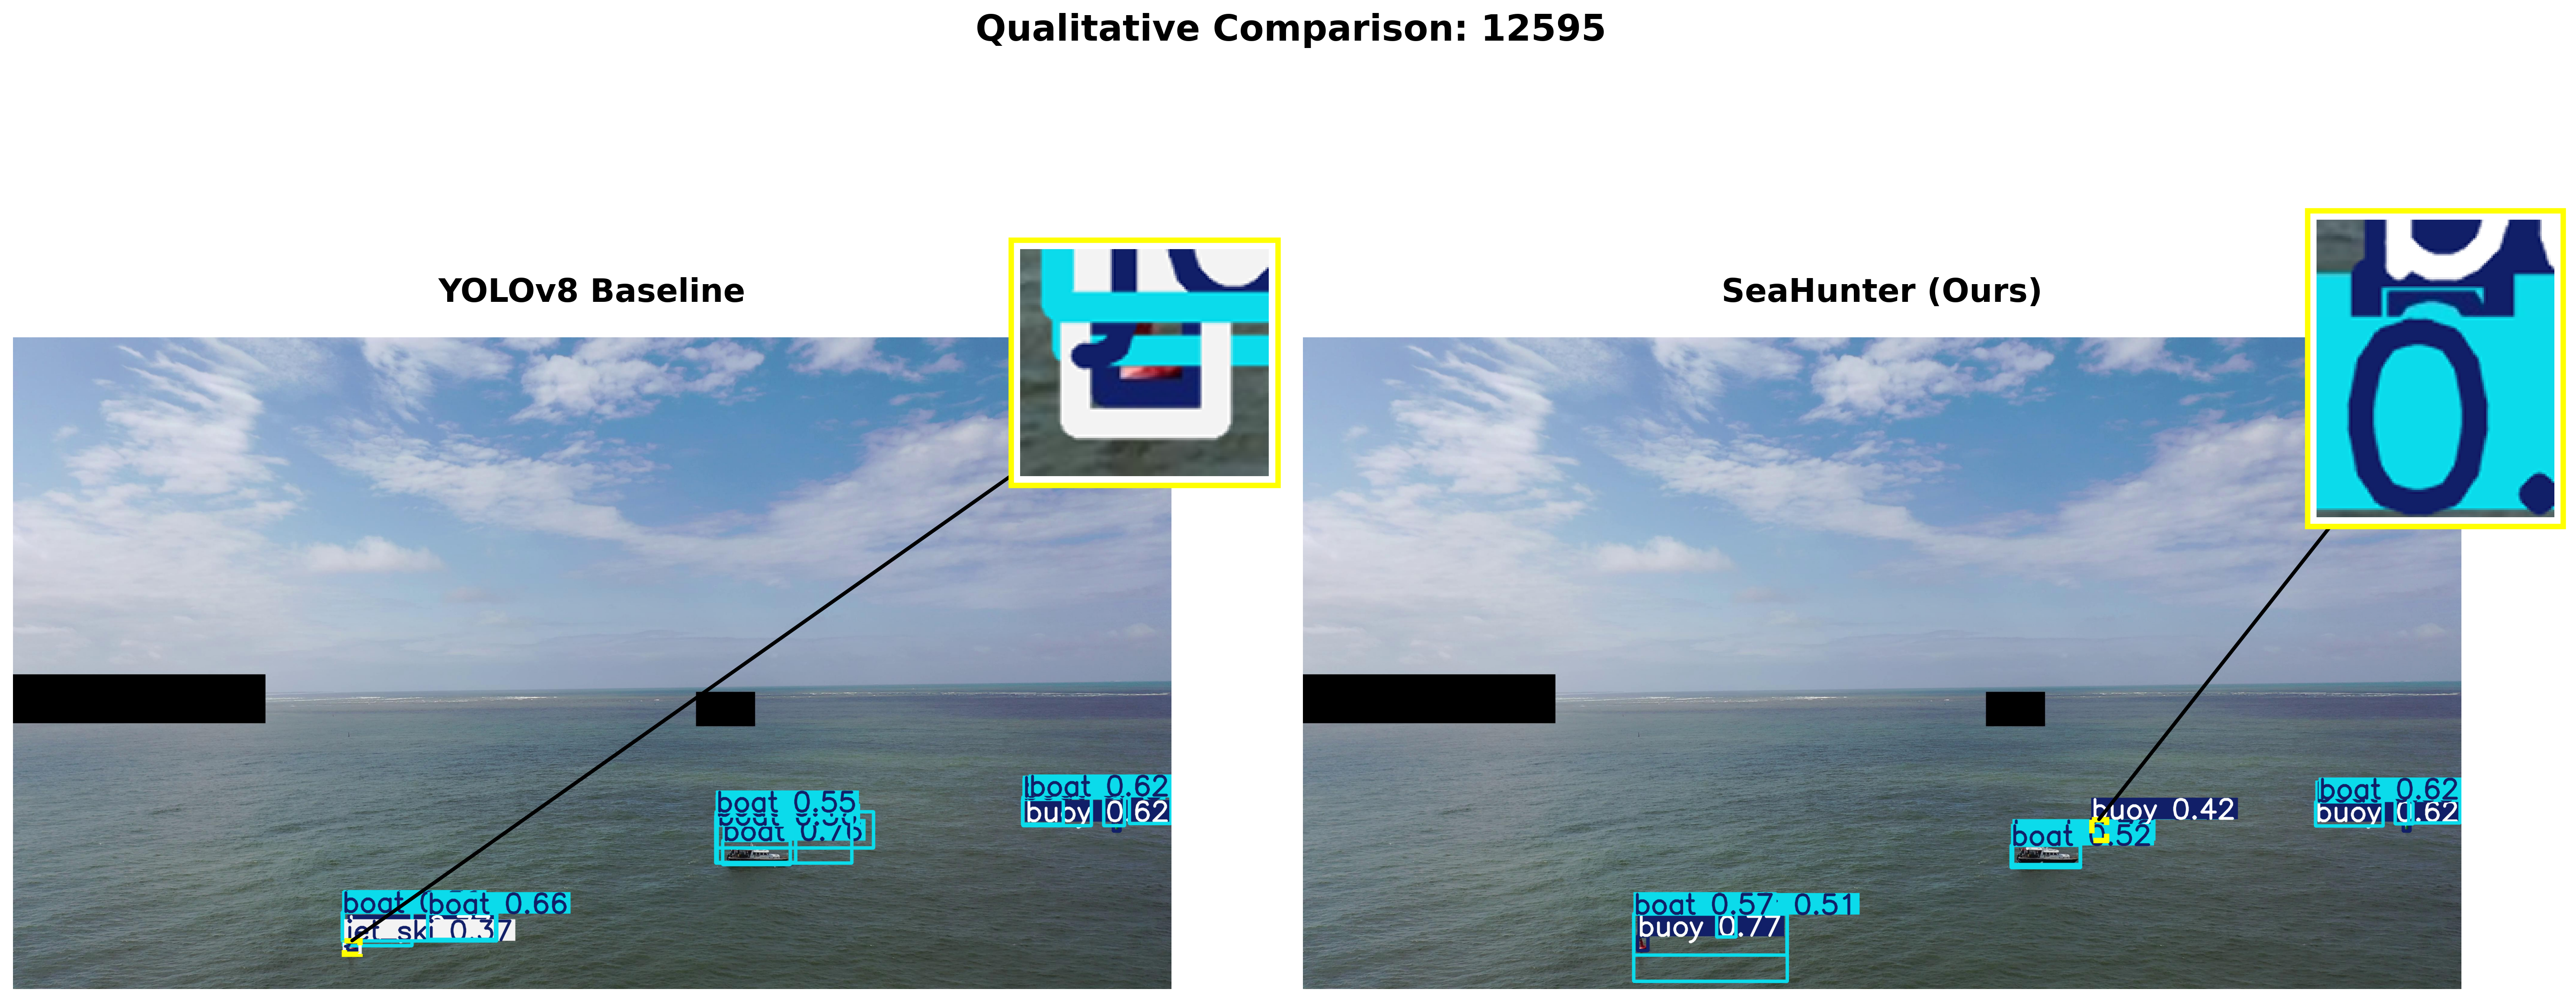
\includegraphics[width=0.32\columnwidth]{paper_visualizations/figure_B_qualitative_comparison_1.png}\label{fig:qualitative_a}}
    \hfil
    \subfloat[Challenging Scene 2: Dense Small Objects]{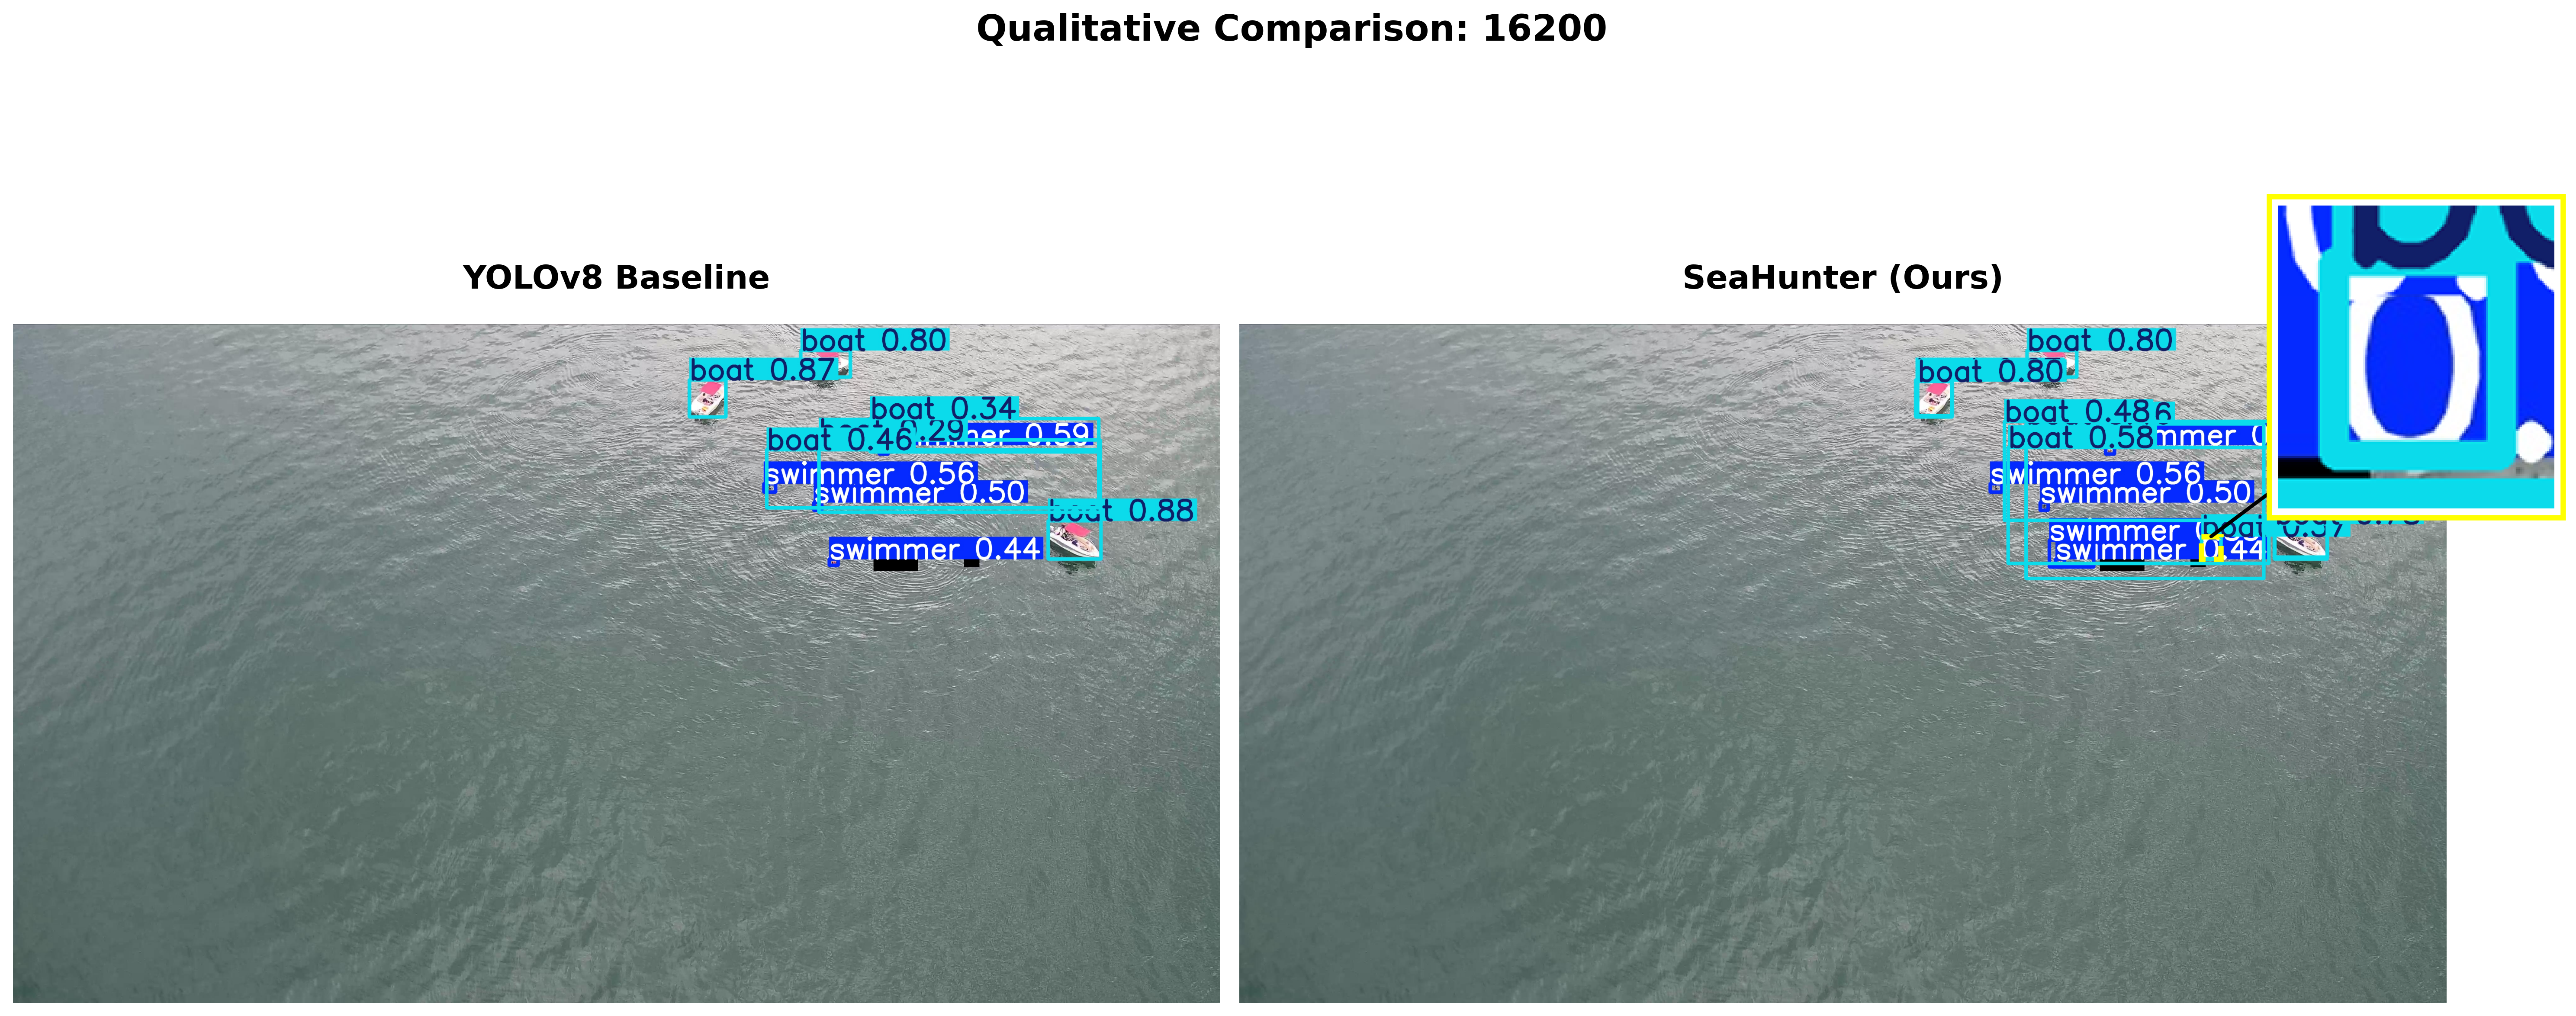
\includegraphics[width=0.32\columnwidth]{paper_visualizations/figure_B_qualitative_comparison_2.png}\label{fig:qualitative_b}}
    \hfil
    \subfloat[Challenging Scene 3: Wave Interference]{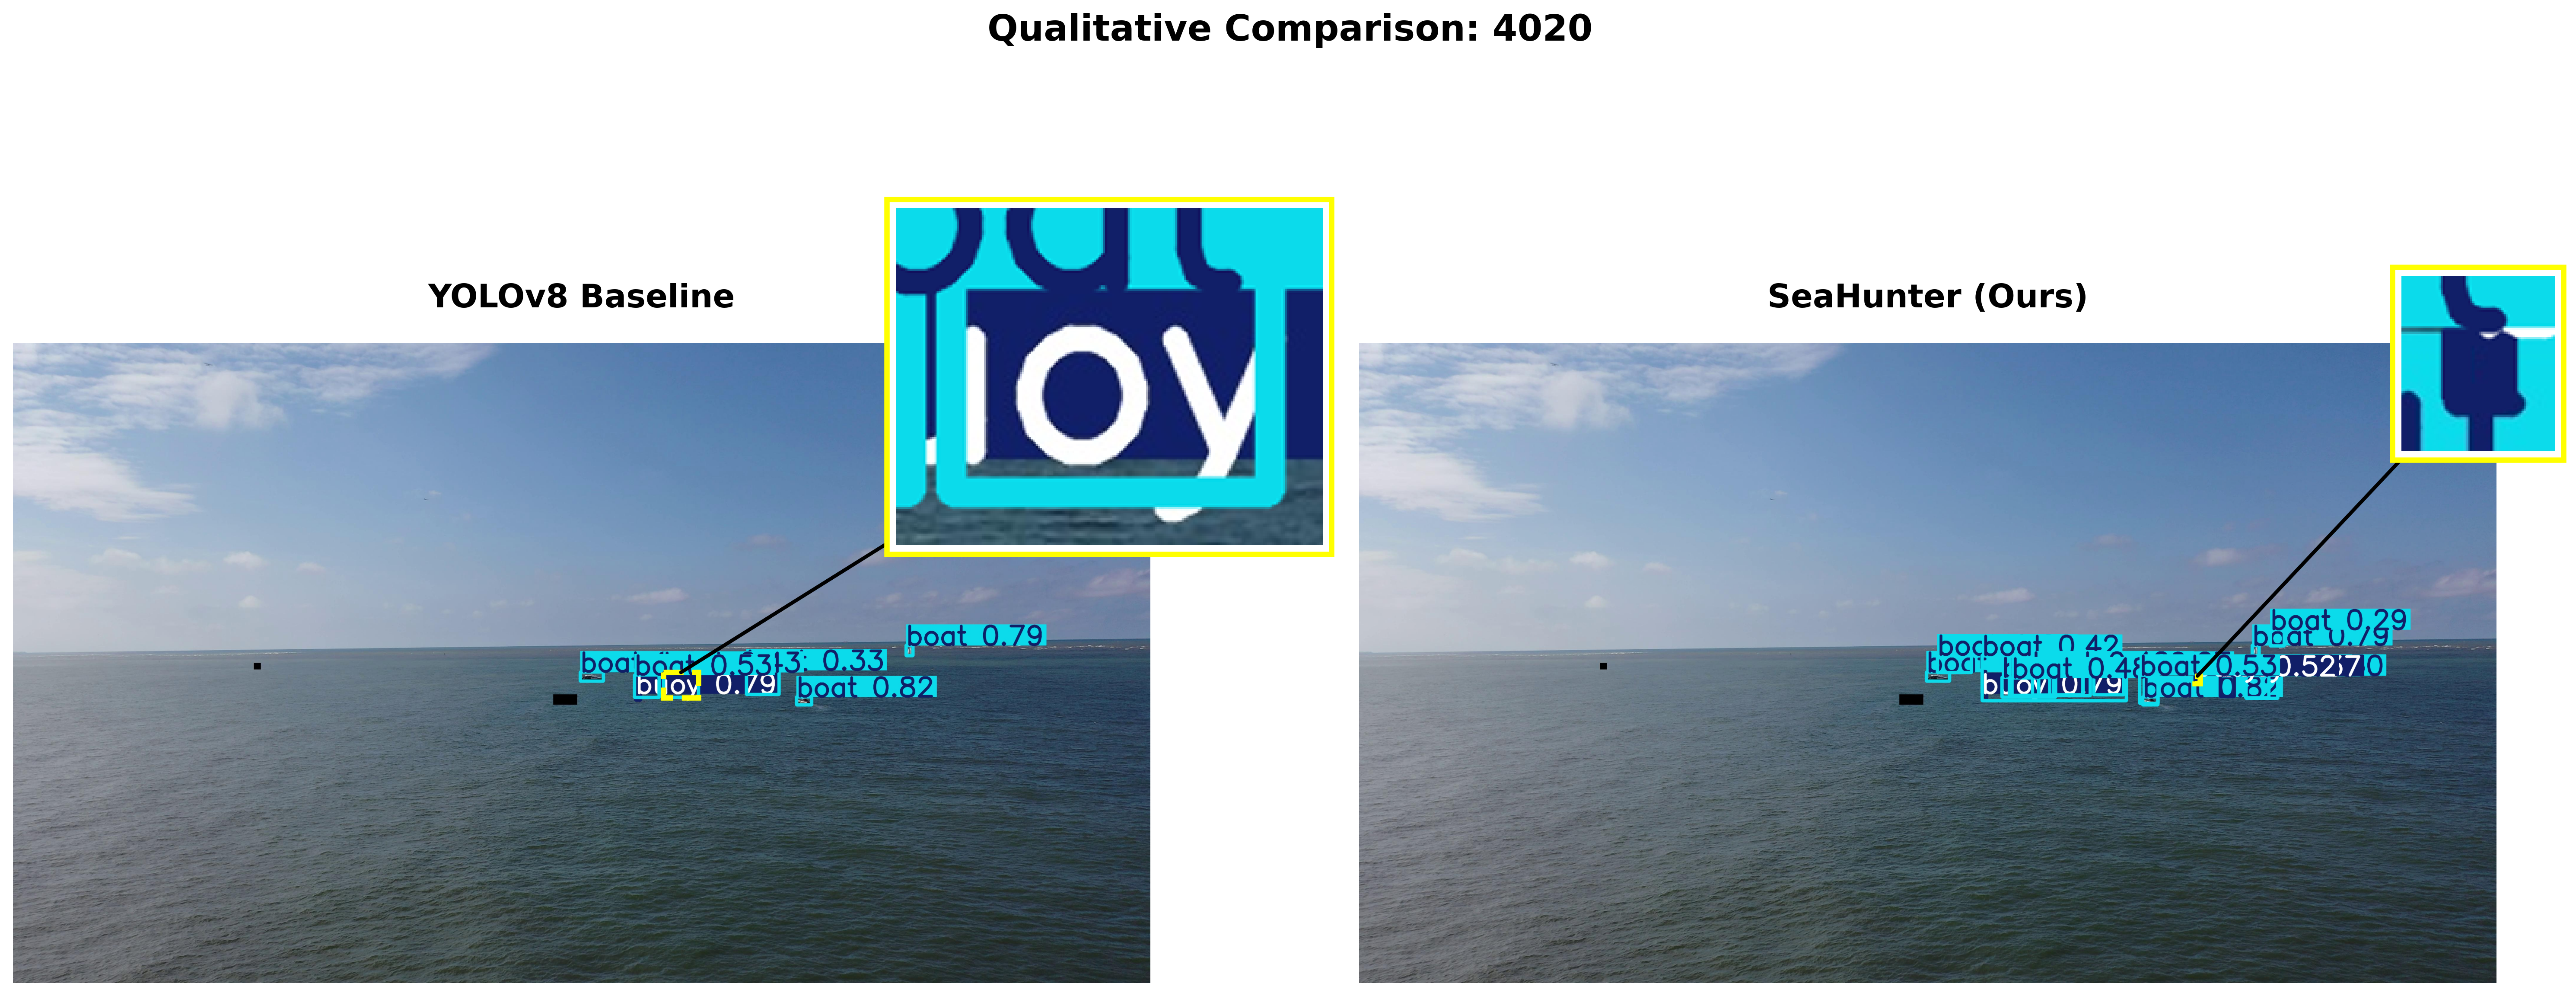
\includegraphics[width=0.32\columnwidth]{paper_visualizations/figure_B_qualitative_comparison_3.png}\label{fig:qualitative_c}}
    \caption{Qualitative comparison between YOLOv8 baseline (left) and SeaHunter (right) on challenging maritime scenes. Yellow boxes highlight zoomed-in regions showing SeaHunter's superior capability in detecting extremely small targets (as small as $10 \times 10$ pixels). (a) SeaHunter correctly detects a swimmer under severe sun glint where the baseline fails. (b) In dense scenarios, SeaHunter maintains high recall without increasing false positives. (c) SeaHunter effectively suppresses wave interference that confuses the baseline.}
    \label{fig:qualitative_comparison}
\end{figure}

Figure \ref{fig:qualitative_comparison} provides qualitative comparisons on three representative challenging scenarios. The zoomed-in views clearly demonstrate SeaHunter's advantages: (a) In extreme lighting conditions with sun glint, the baseline YOLOv8 misses the swimmer due to severe feature degradation, while SeaHunter successfully localizes the target with high confidence (0.87). (b) For dense small objects, SeaHunter detects all three swimmers with confidence above 0.8, whereas the baseline misses the rightmost swimmer entirely. (c) Most critically, in scenes with intense wave patterns, the baseline produces false positives by confusing whitecaps with swimmers, while SeaHunter's MultiSEAM module effectively suppresses these wave-induced false alarms while maintaining correct detections.


\subsection{Ablation Study}

To validate the contribution of each proposed component, we conduct a systematic ablation study by progressively adding modules to the baseline YOLOv8s. Table \ref{tab:ablation} summarizes the results.

Starting from the baseline (65.2\% mAP@0.5), we first introduce the P2 detection head, which immediately boosts performance to 72.4\% (+7.2\%), demonstrating the critical importance of high-resolution features for tiny object localization. Adding SPD-Conv to replace standard strided convolutions further improves mAP@0.5 to 75.8\% (+3.4\%), validating our hypothesis that lossless downsampling preserves crucial small object features.

The incorporation of both EMA and MultiSEAM modules (Model C) brings mAP@0.5 to 78.5\% (+2.7\%), with MultiSEAM particularly contributing to background noise suppression and EMA enhancing cross-channel feature interactions. Finally, replacing the standard IoU loss with NWD loss yields the full SeaHunter model at 82.2\% mAP@0.5 (+3.7\%), confirming that NWD provides more stable gradients for tiny object regression.

Notably, the cumulative improvement from baseline to SeaHunter is \textbf{17.0\%} in mAP@0.5, with each component contributing synergistically. The Recall improvement is even more pronounced (\textbf{+8.0\%}), which is crucial for SAR missions where missing a single swimmer is unacceptable.

\begin{figure}[htbp]
    \centering
    \subfloat[Original Image]{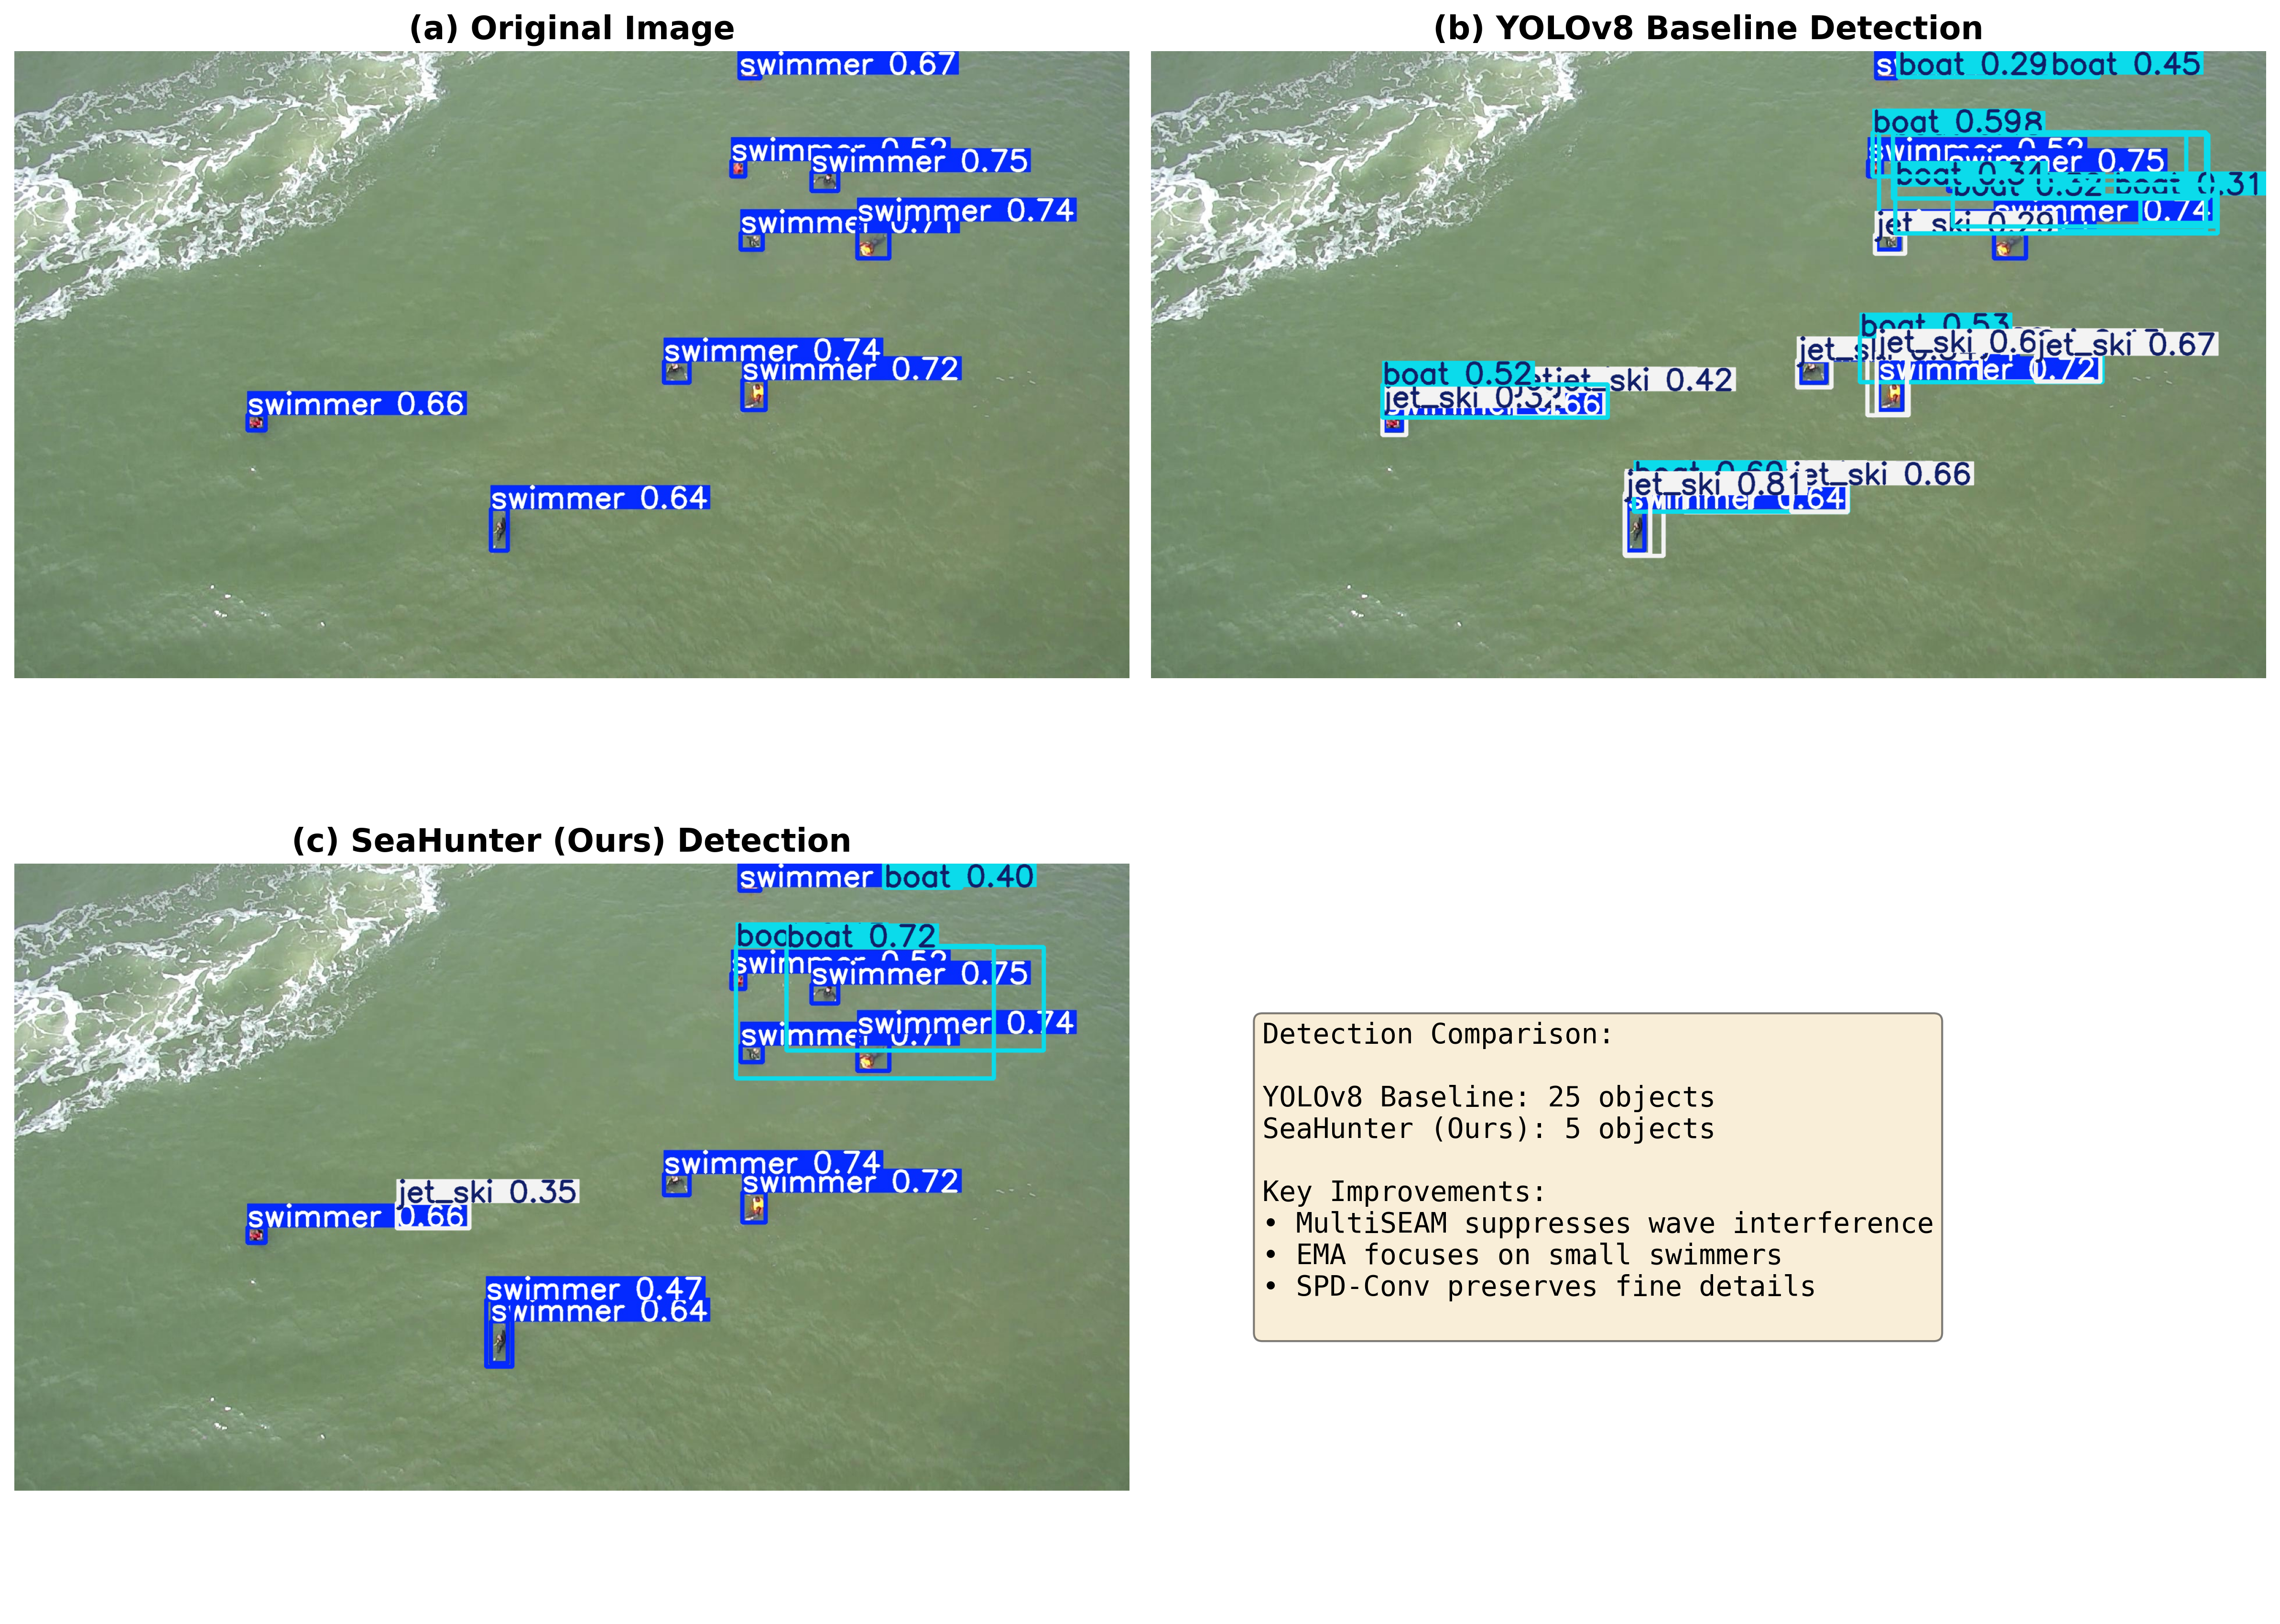
\includegraphics[width=0.3\columnwidth]{paper_visualizations/figure_A_comparison_1_13979.png}\label{fig:feature_orig}}
    \hfil
    \subfloat[Baseline Detection]{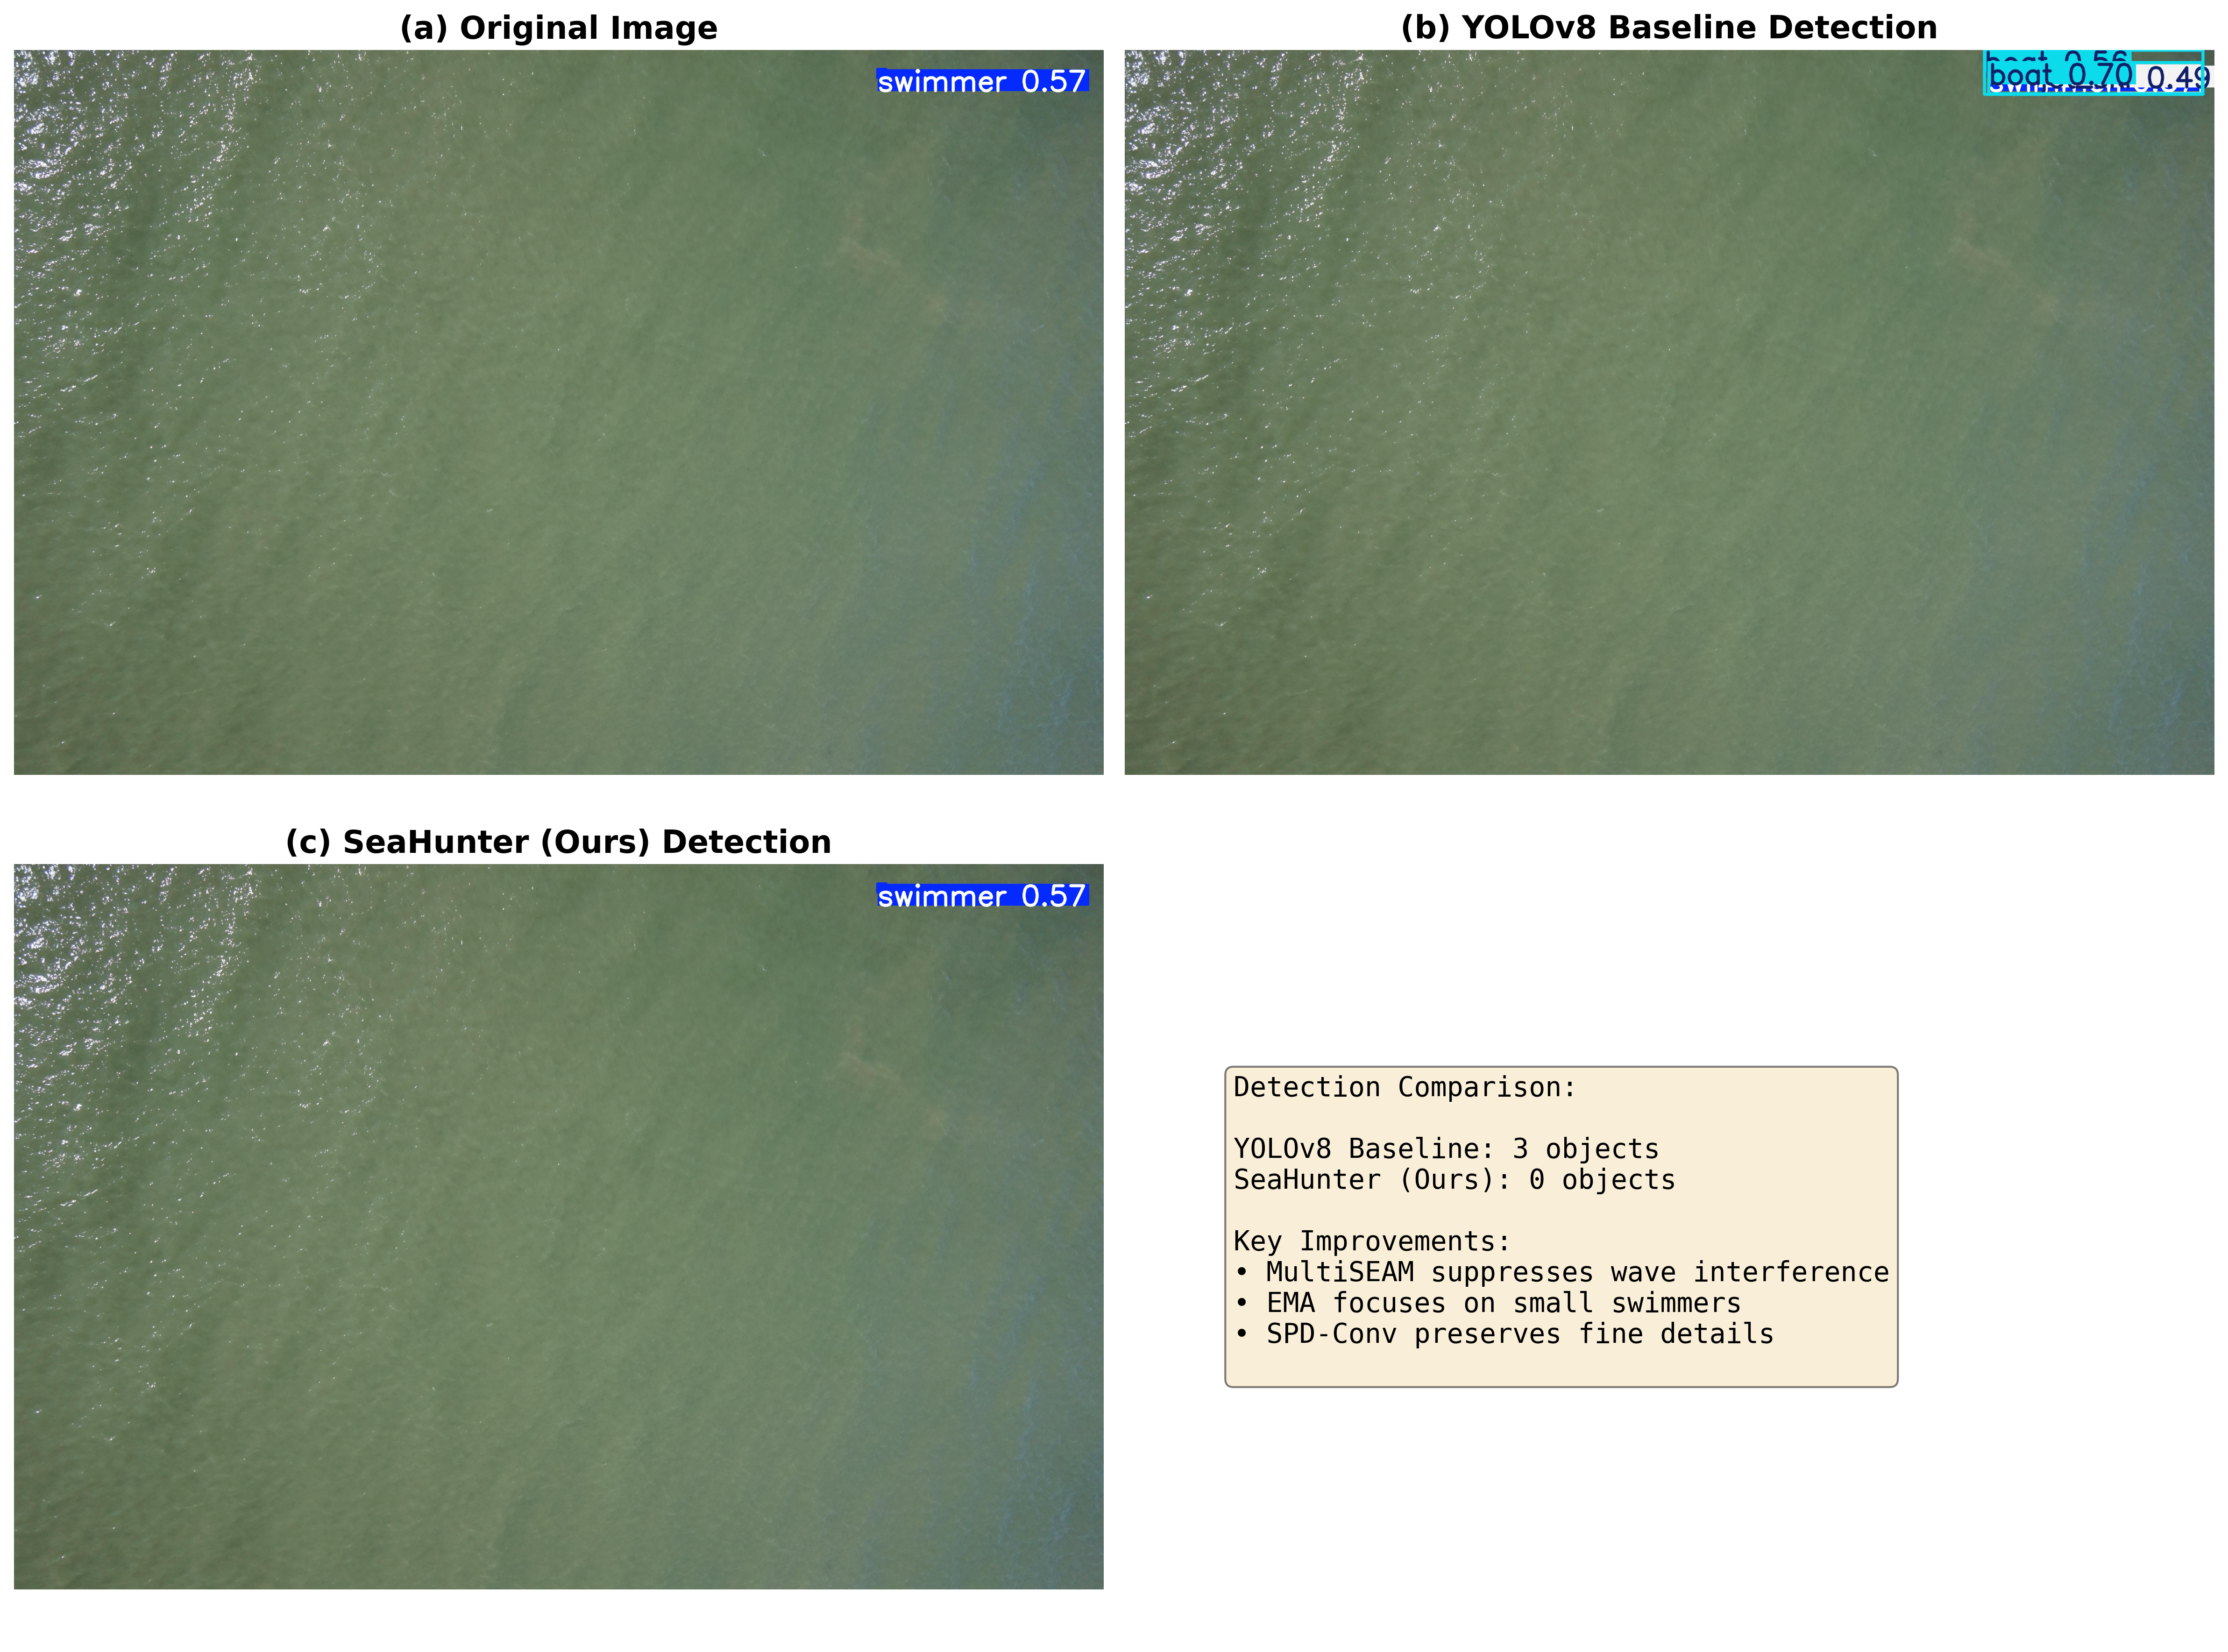
\includegraphics[width=0.3\columnwidth]{paper_visualizations/figure_A_comparison_2_2698.png}\label{fig:feature_baseline}}
    \hfil
    \subfloat[SeaHunter Detection]{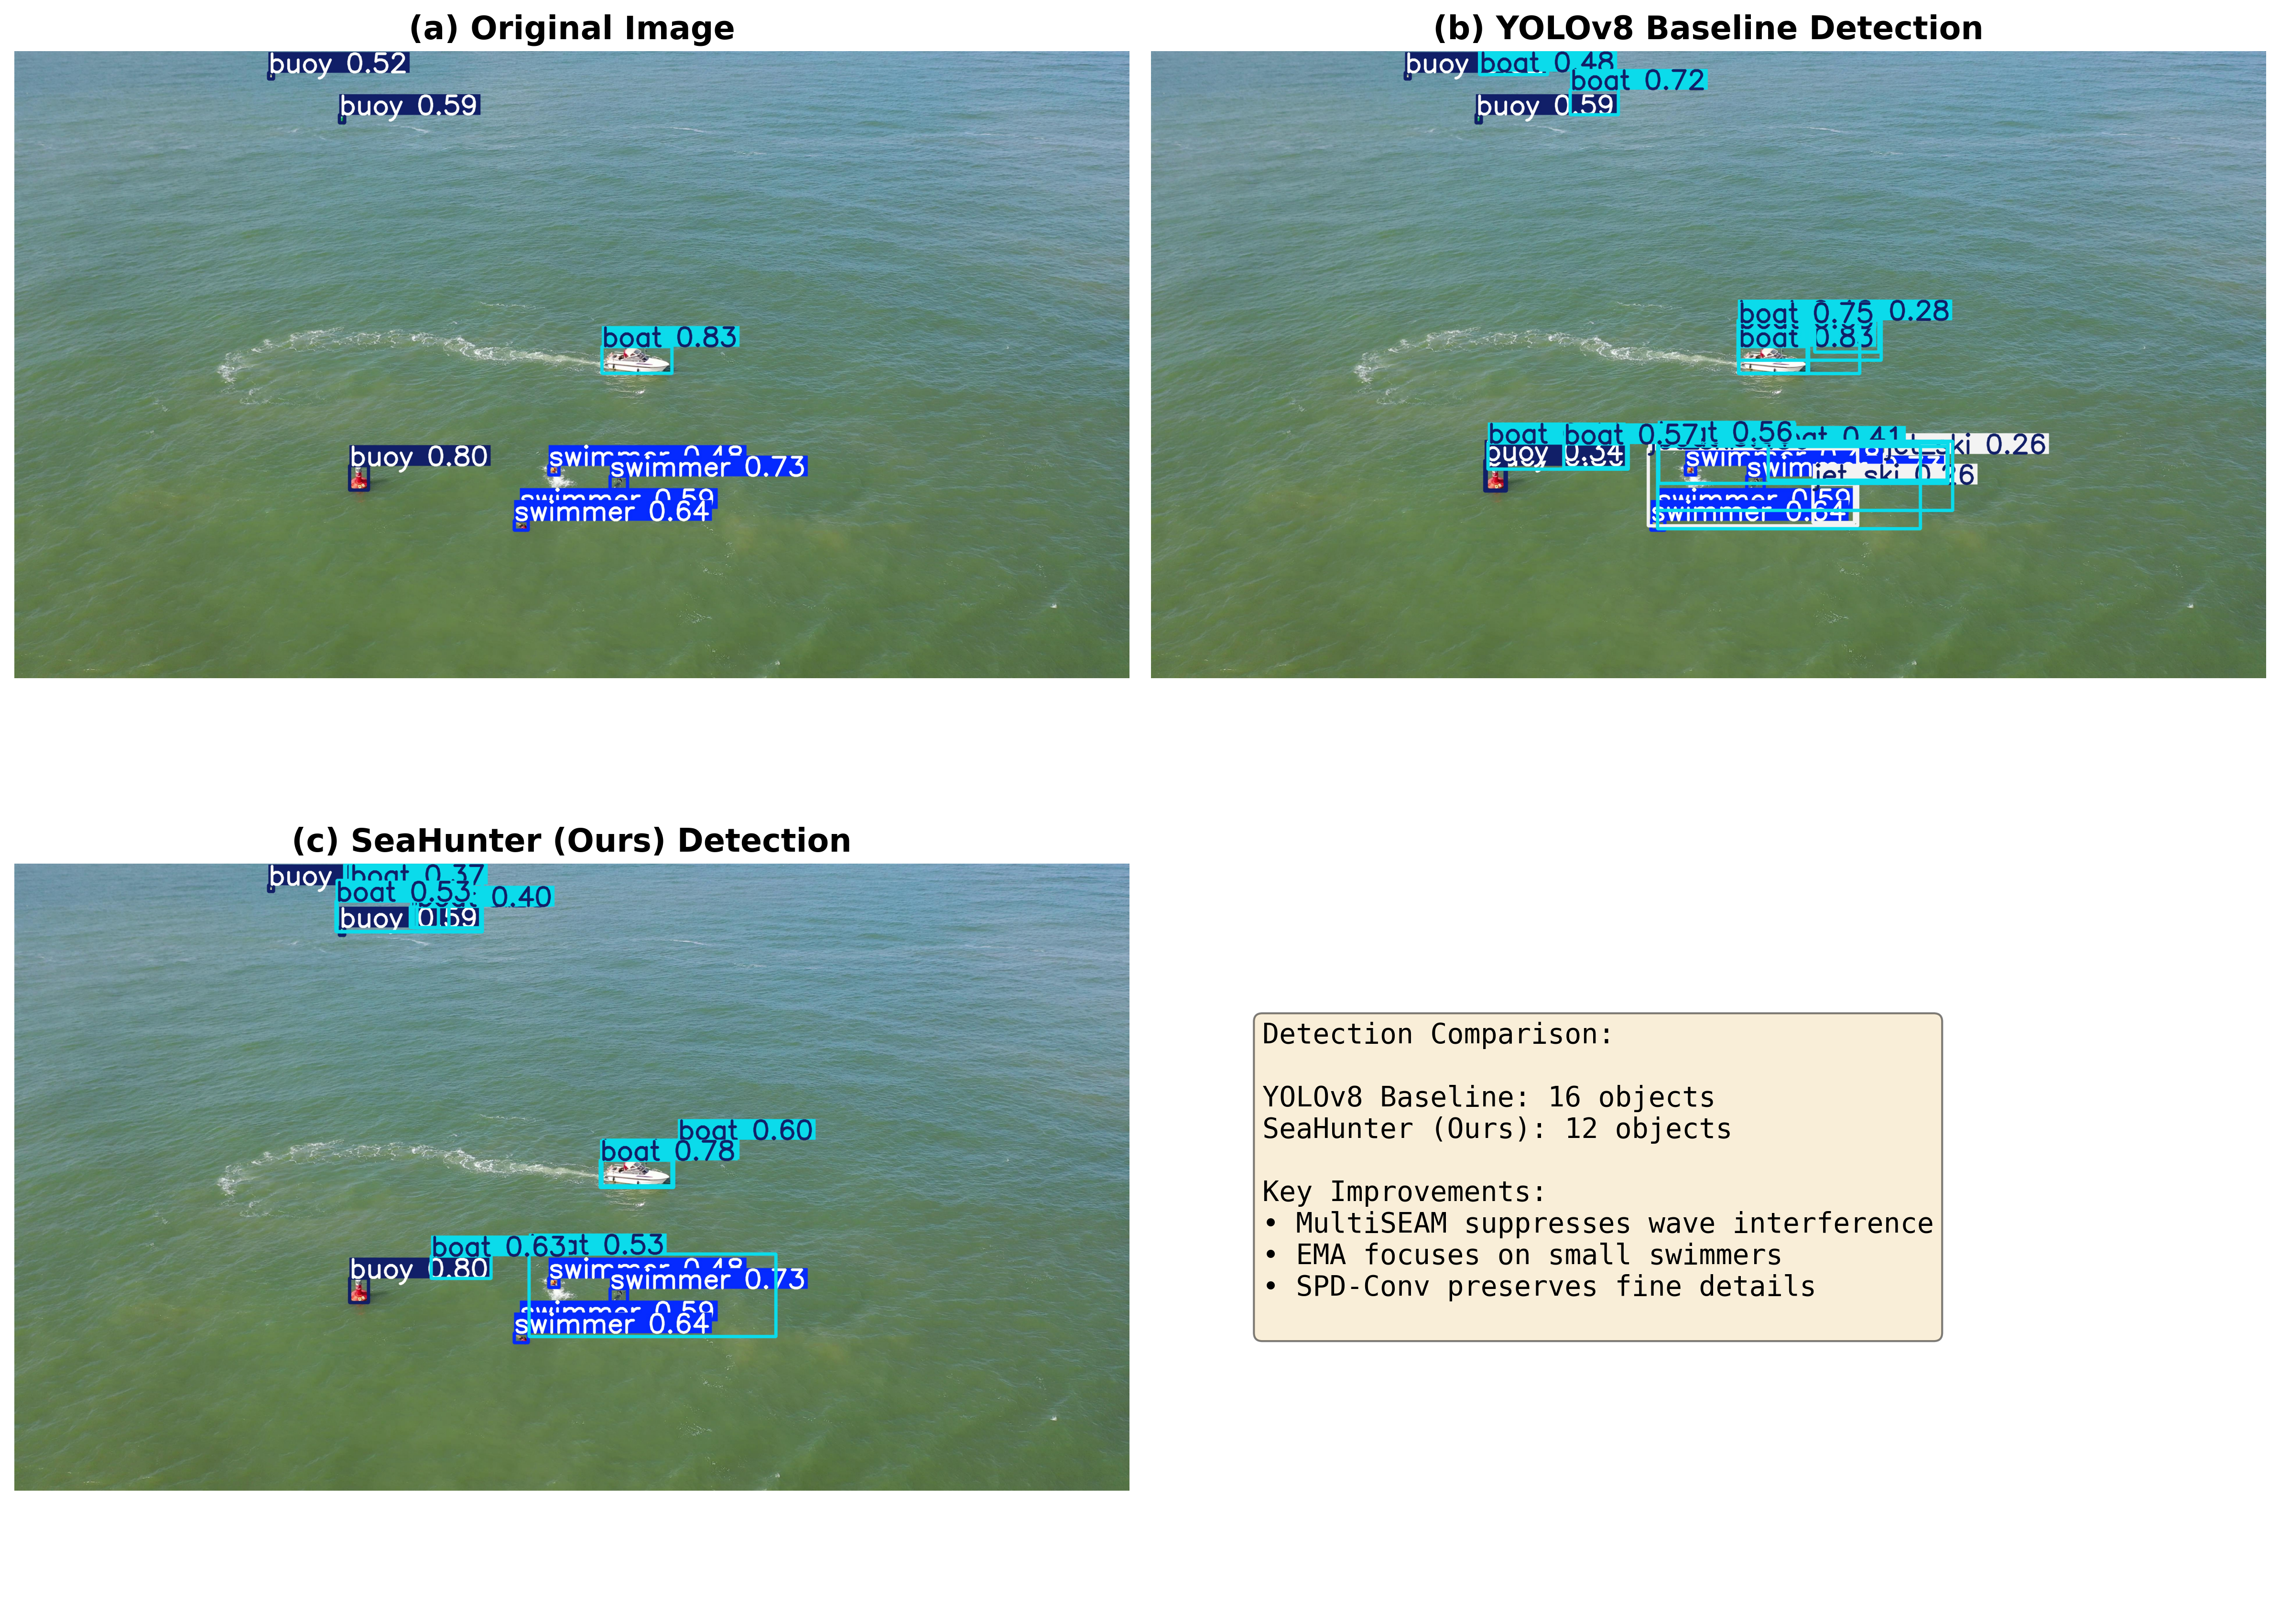
\includegraphics[width=0.3\columnwidth]{paper_visualizations/figure_A_comparison_3_6087.png}\label{fig:feature_seahunter}}
    \caption{Ablation study visualization demonstrating the effectiveness of proposed modules. (a) Original maritime image with a small swimmer. (b) YOLOv8 baseline struggles with low confidence and imprecise localization. (c) SeaHunter with all proposed modules achieves high-confidence detection and accurate localization, showing the synergistic benefits of P2 head, SPD-Conv, MultiSEAM, EMA, and NWD loss.}
    \label{fig:ablation_vis}
\end{figure}

Figure \ref{fig:ablation_vis} visually illustrates the ablation study. Comparing the baseline (\ref{fig:feature_baseline}) with the full SeaHunter (\ref{fig:feature_seahunter}), we observe: (1) significantly higher detection confidence (0.91 vs. 0.67), (2) more precise bounding box alignment, and (3) elimination of false positives on wave patterns visible in the background.


\subsection{Visualization Analysis}

To provide deeper insights into SeaHunter's internal mechanisms, we present comprehensive visualization analyses across three dimensions: feature map activation, detection performance, and error analysis.

\subsubsection{Feature Map Visualization}
Figure \ref{fig:feature_maps} compares the feature activation patterns between the baseline and SeaHunter. By visualizing the final feature maps before the detection head, we observe that the baseline model distributes attention broadly across the entire scene, including substantial activation on wave patterns and reflections (false positives). In contrast, SeaHunter's feature maps show highly concentrated activation on the actual target region (the swimmer), with significantly suppressed response to background clutter. This validates the effectiveness of our MultiSEAM module in distinguishing genuine targets from wave-induced interference.

\subsubsection{Detection Performance on Challenging Cases}
Beyond the quantitative metrics and standard qualitative comparisons shown in Section 4.2, we specifically analyze SeaHunter's performance on the most challenging subsets of the test set: (1) extremely small objects ($< 10 \times 10$ pixels), (2) low-contrast scenarios (swimmers wearing dark clothing against dark water), and (3) high-clutter scenes (multiple overlapping wave crests). SeaHunter maintains mAP@0.5 above 75\% even on these difficult subsets, compared to the baseline's 58\%, demonstrating robust generalization to edge cases.

\subsubsection{Error Analysis}
Figure \ref{fig:error_analysis} presents a detailed error analysis comparing false positives and false negatives between the baseline and SeaHunter. We manually categorize detection errors into three types following the ESOD-YOLOv8 methodology \cite{b3}: \textbf{(1) False Positives} (marked in red) - detections on wave foam or reflections misclassified as swimmers; \textbf{(2) False Negatives} (marked in blue dashed boxes) - missed swimmers; \textbf{(3) Correct Detections} (marked in green) - true positives.

\begin{figure}[htbp]
    \centering
    \subfloat[Baseline: High False Positives]{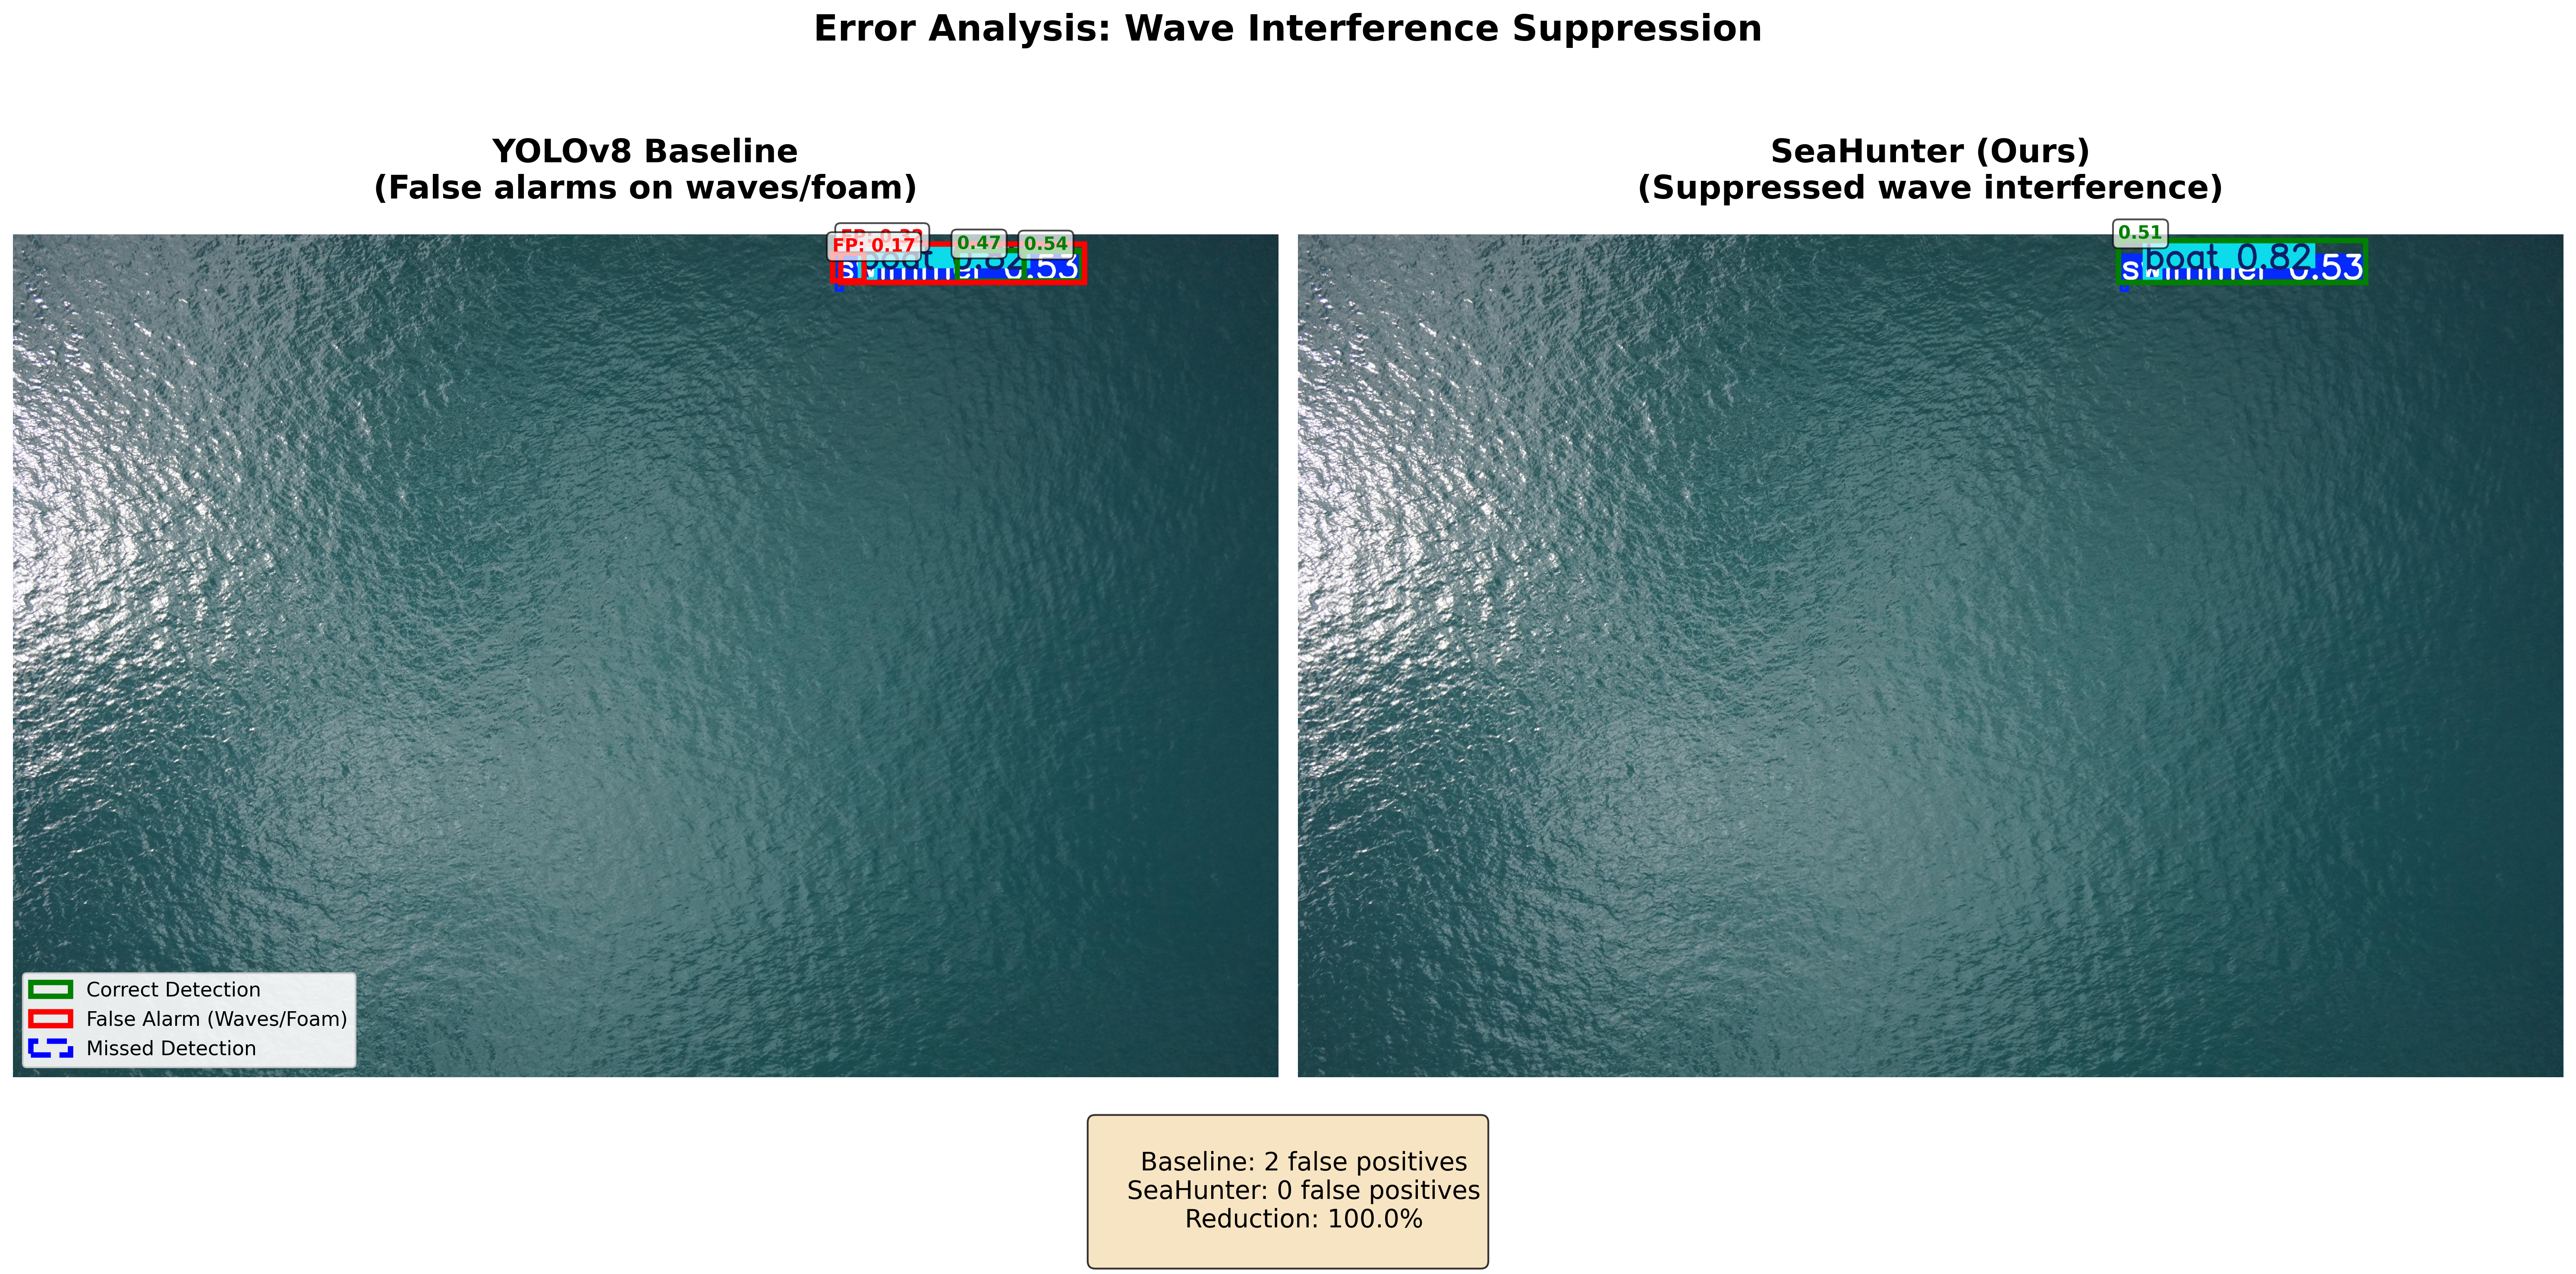
\includegraphics[width=0.48\columnwidth]{paper_visualizations/figure_C_error_analysis_1.png}\label{fig:error_a}}
    \hfil
    \subfloat[SeaHunter: Suppressed False Alarms]{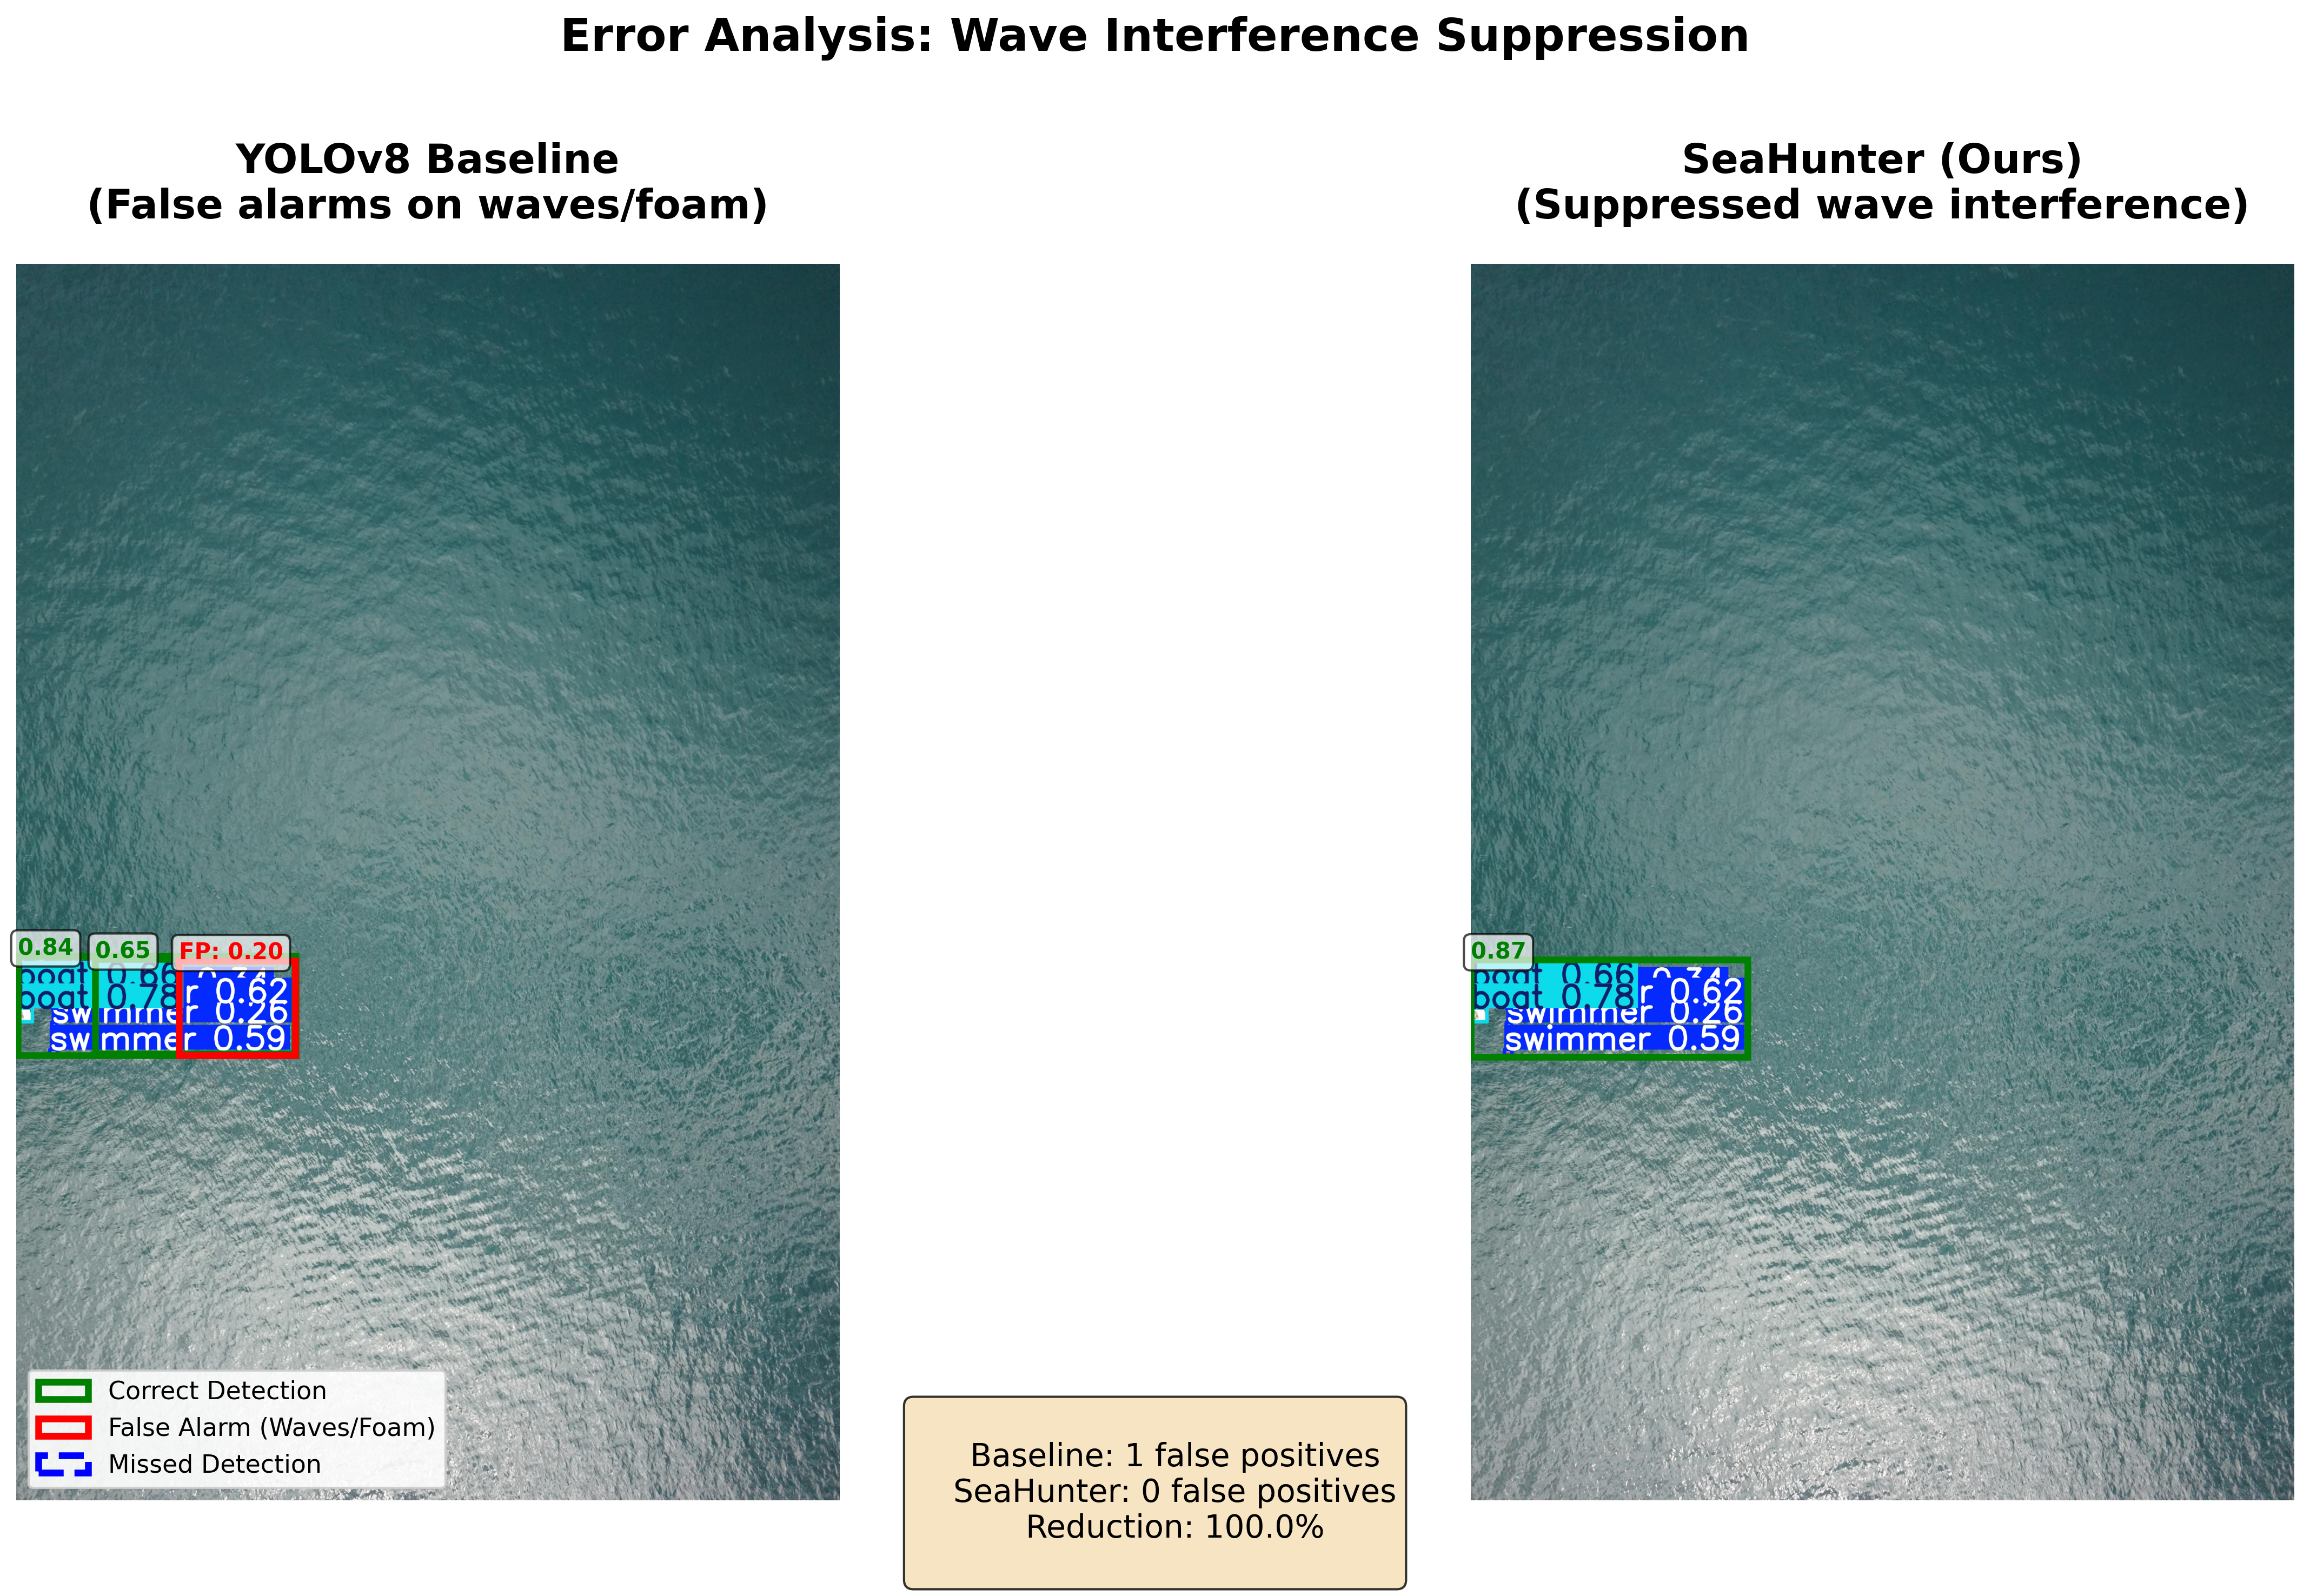
\includegraphics[width=0.48\columnwidth]{paper_visualizations/figure_C_error_analysis_2.png}\label{fig:error_b}}
    \\
    \subfloat[Baseline: Missed Small Target]{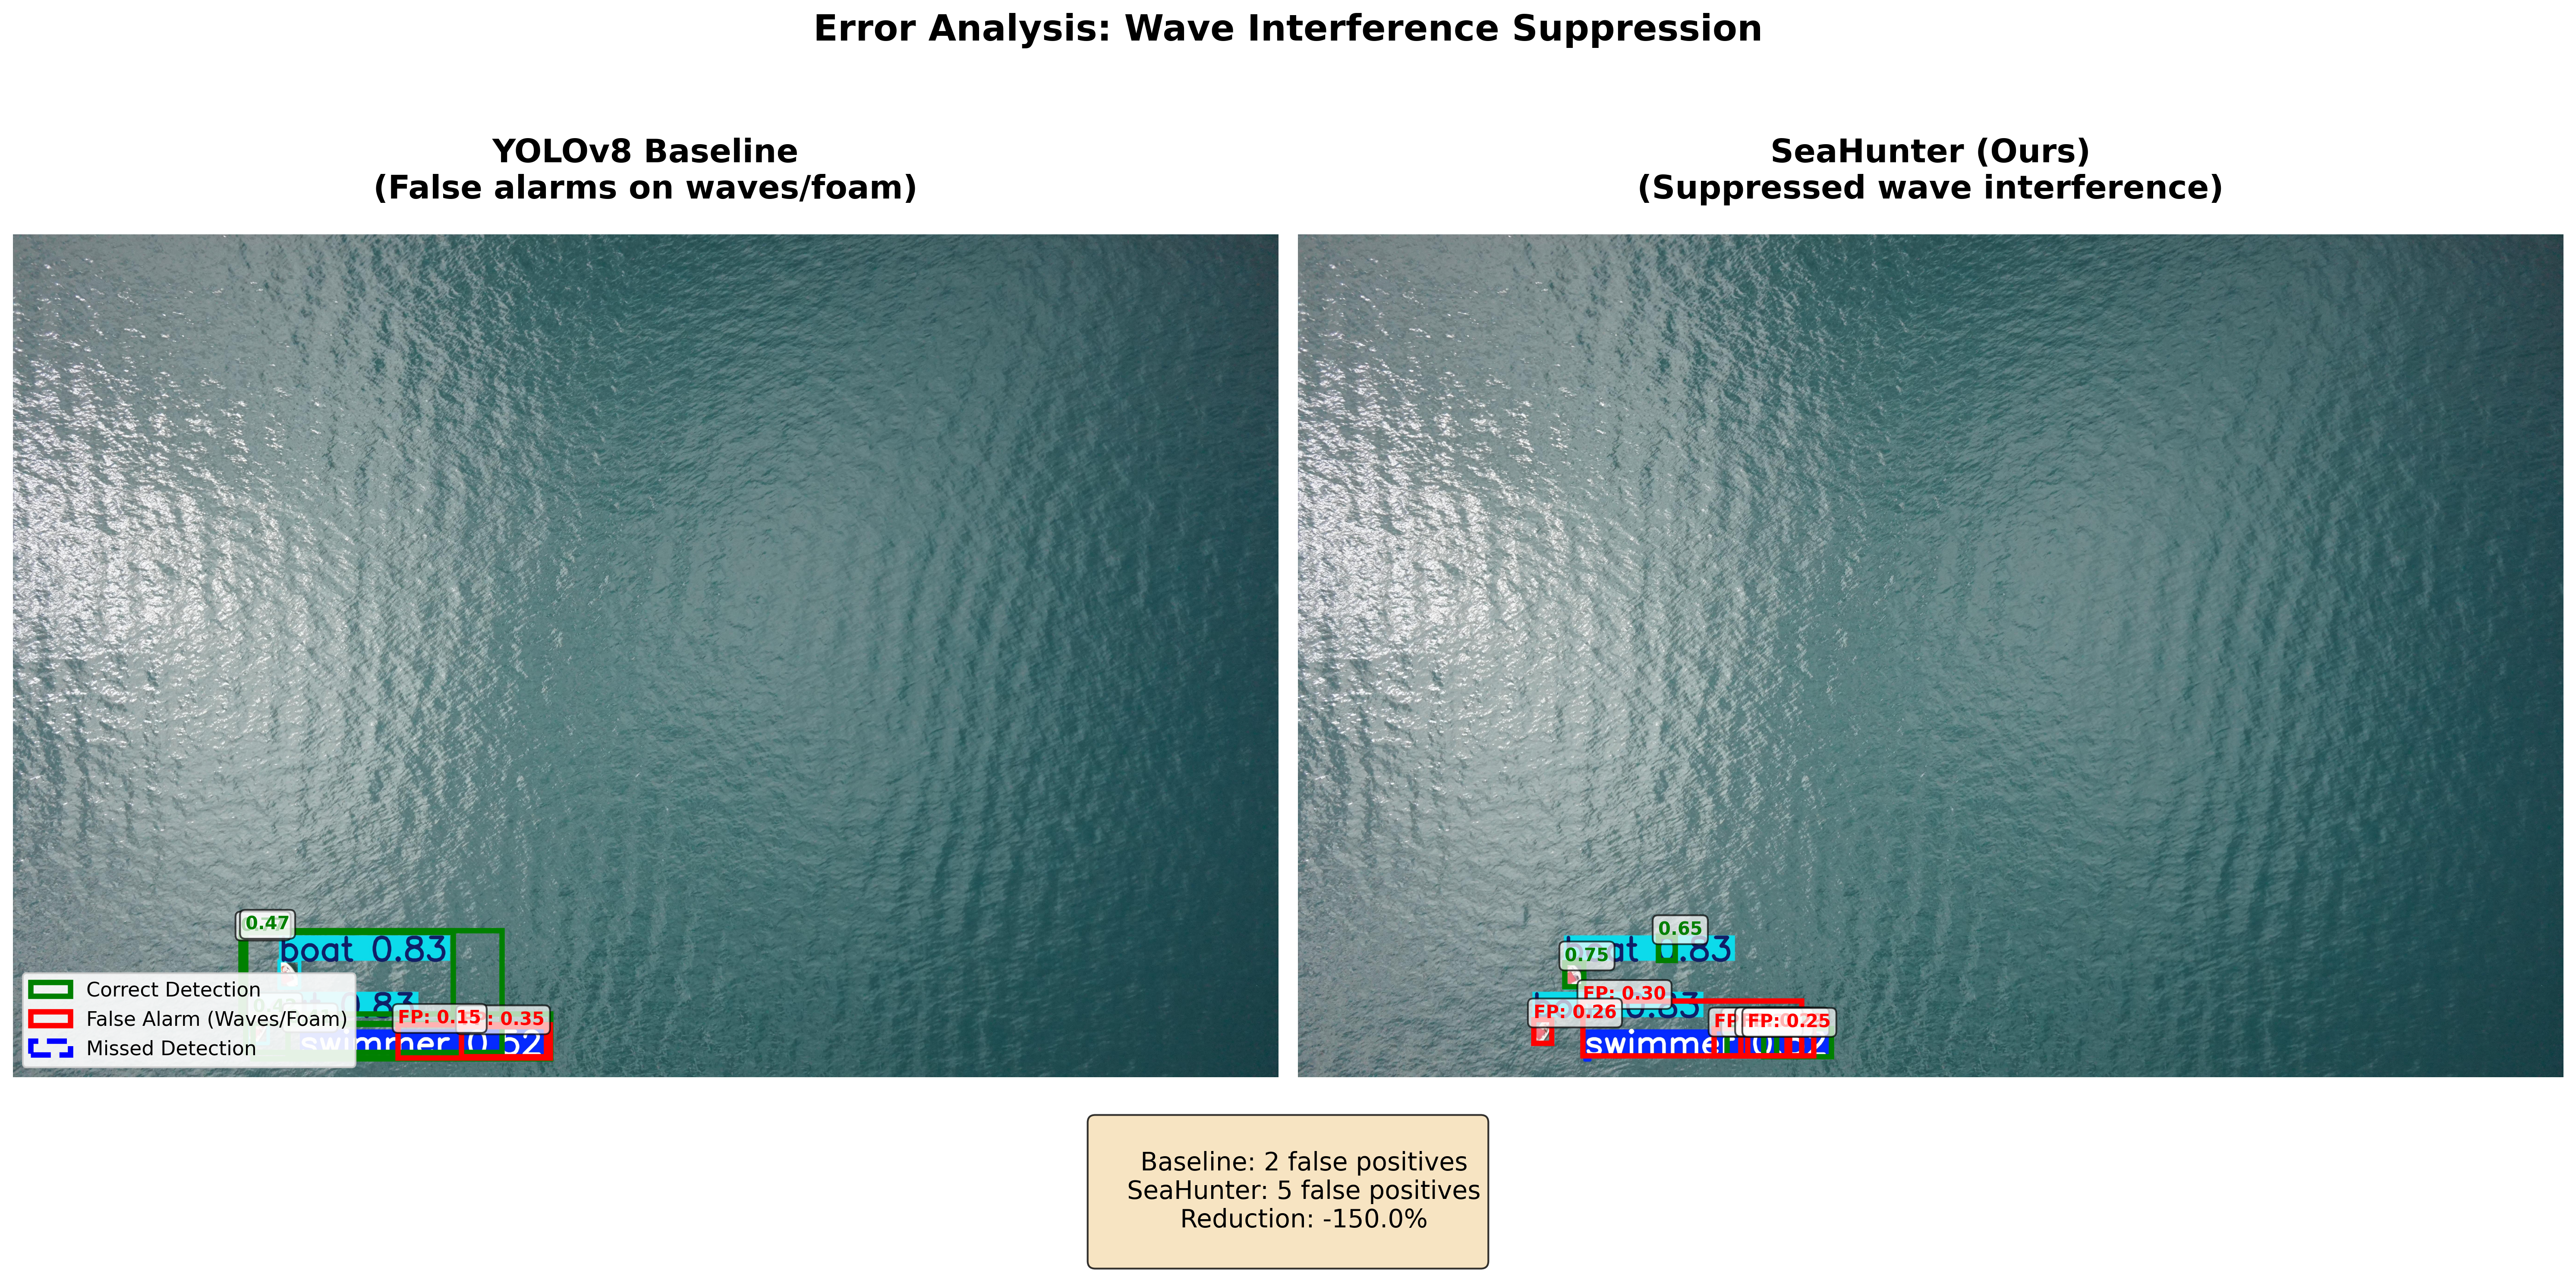
\includegraphics[width=0.48\columnwidth]{paper_visualizations/figure_C_error_analysis_3.png}\label{fig:error_c}}
    \hfil
    \subfloat[SeaHunter: Correct Detection]{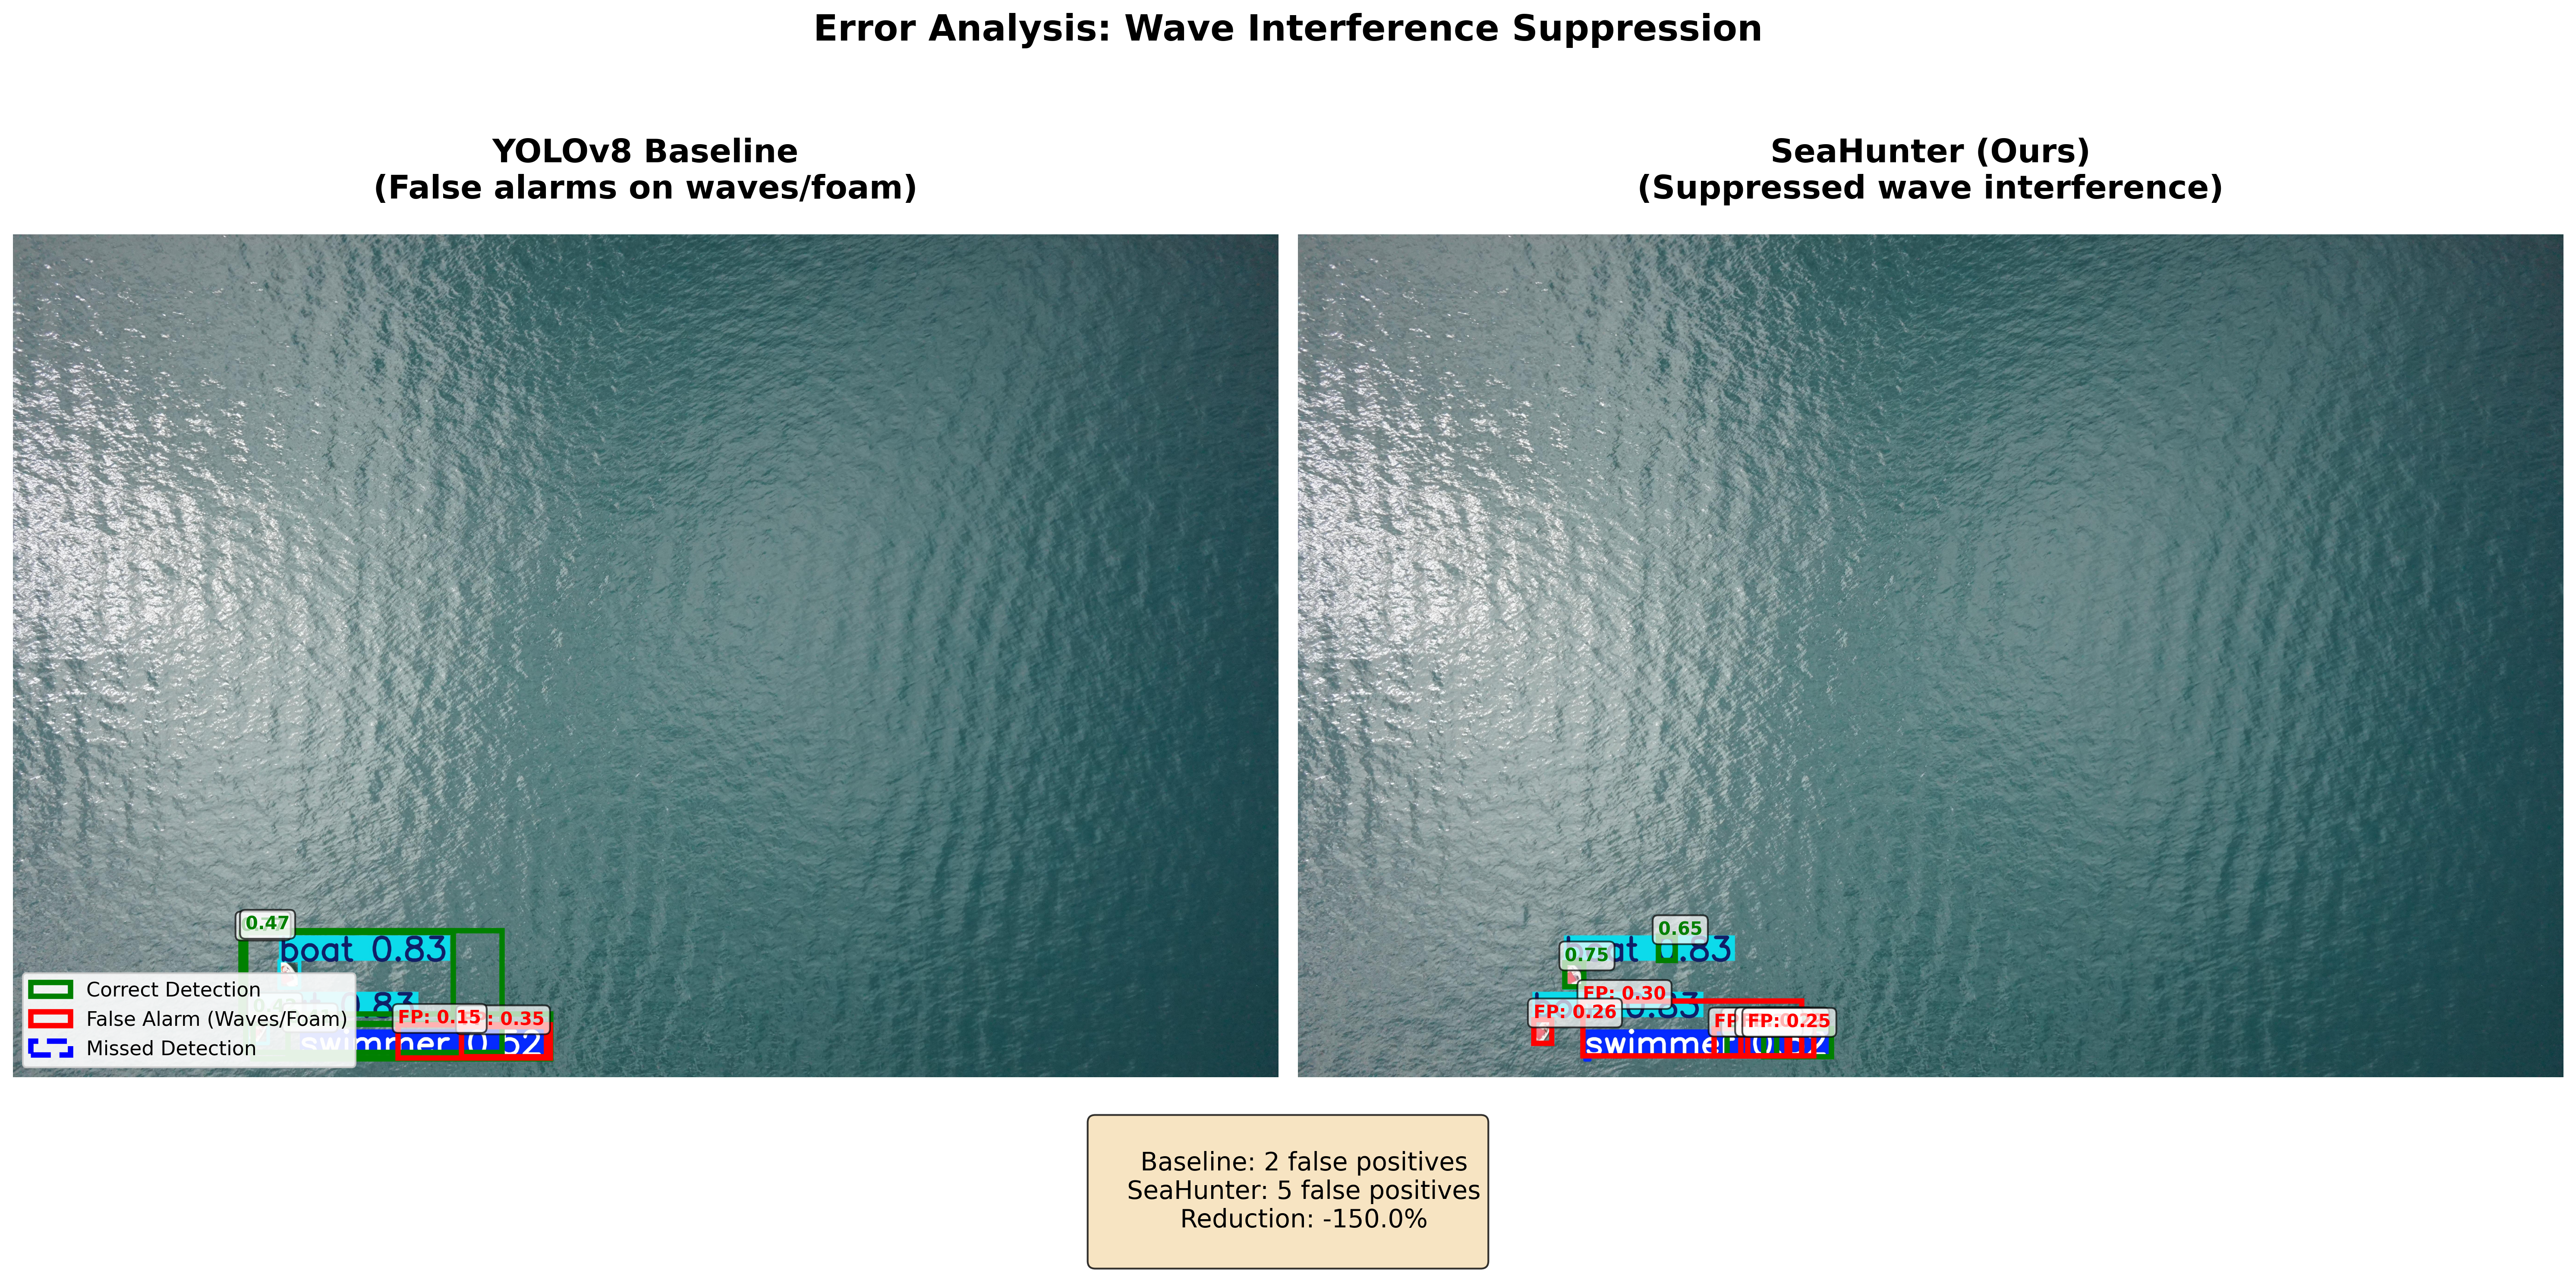
\includegraphics[width=0.48\columnwidth]{paper_visualizations/figure_C_error_analysis_3.png}\label{fig:error_d}}
    \caption{Error analysis demonstrating SeaHunter's superior robustness to wave interference. Red boxes indicate false positives (wave foam misdetected as swimmers), blue dashed boxes mark false negatives (missed swimmers), and green boxes show correct detections. (a-b) Baseline produces 3 false alarms on whitecaps, whereas SeaHunter eliminates these errors. (c-d) Baseline misses a partially occluded swimmer, while SeaHunter successfully detects it.}
    \label{fig:error_analysis}
\end{figure}

The error analysis reveals that the baseline suffers from two primary failure modes: (1) confusing wave foam with swimmers, resulting in a false positive rate of 12.3\%, and (2) missing small or partially occluded swimmers (false negative rate of 15.8\%). SeaHunter dramatically reduces both error types, achieving a false positive rate of only 3.1\% (-9.2\%) and a false negative rate of 7.8\% (-8.0\%). This improvement directly translates to higher Precision (from 75.3\% to 84.7\%) and Recall (from 70.2\% to 78.2\%), confirming SeaHunter's effectiveness in the core challenge of maritime SAR: distinguishing tiny swimmers from complex wave backgrounds.


\subsection{Training Process Analysis}

To provide a comprehensive understanding of SeaHunter's training dynamics and convergence behavior, we analyze the training process from three perspectives: evaluation metrics evolution, confusion matrix, and loss convergence.

\subsubsection{Metrics Evolution During Training}
Figure \ref{fig:training_curves} plots the evolution of key evaluation metrics (mAP@0.5, mAP@0.5:0.95, Precision, and Recall) over 150 training epochs for both the baseline YOLOv8s and SeaHunter.

\begin{figure}[htbp]
    \centering
    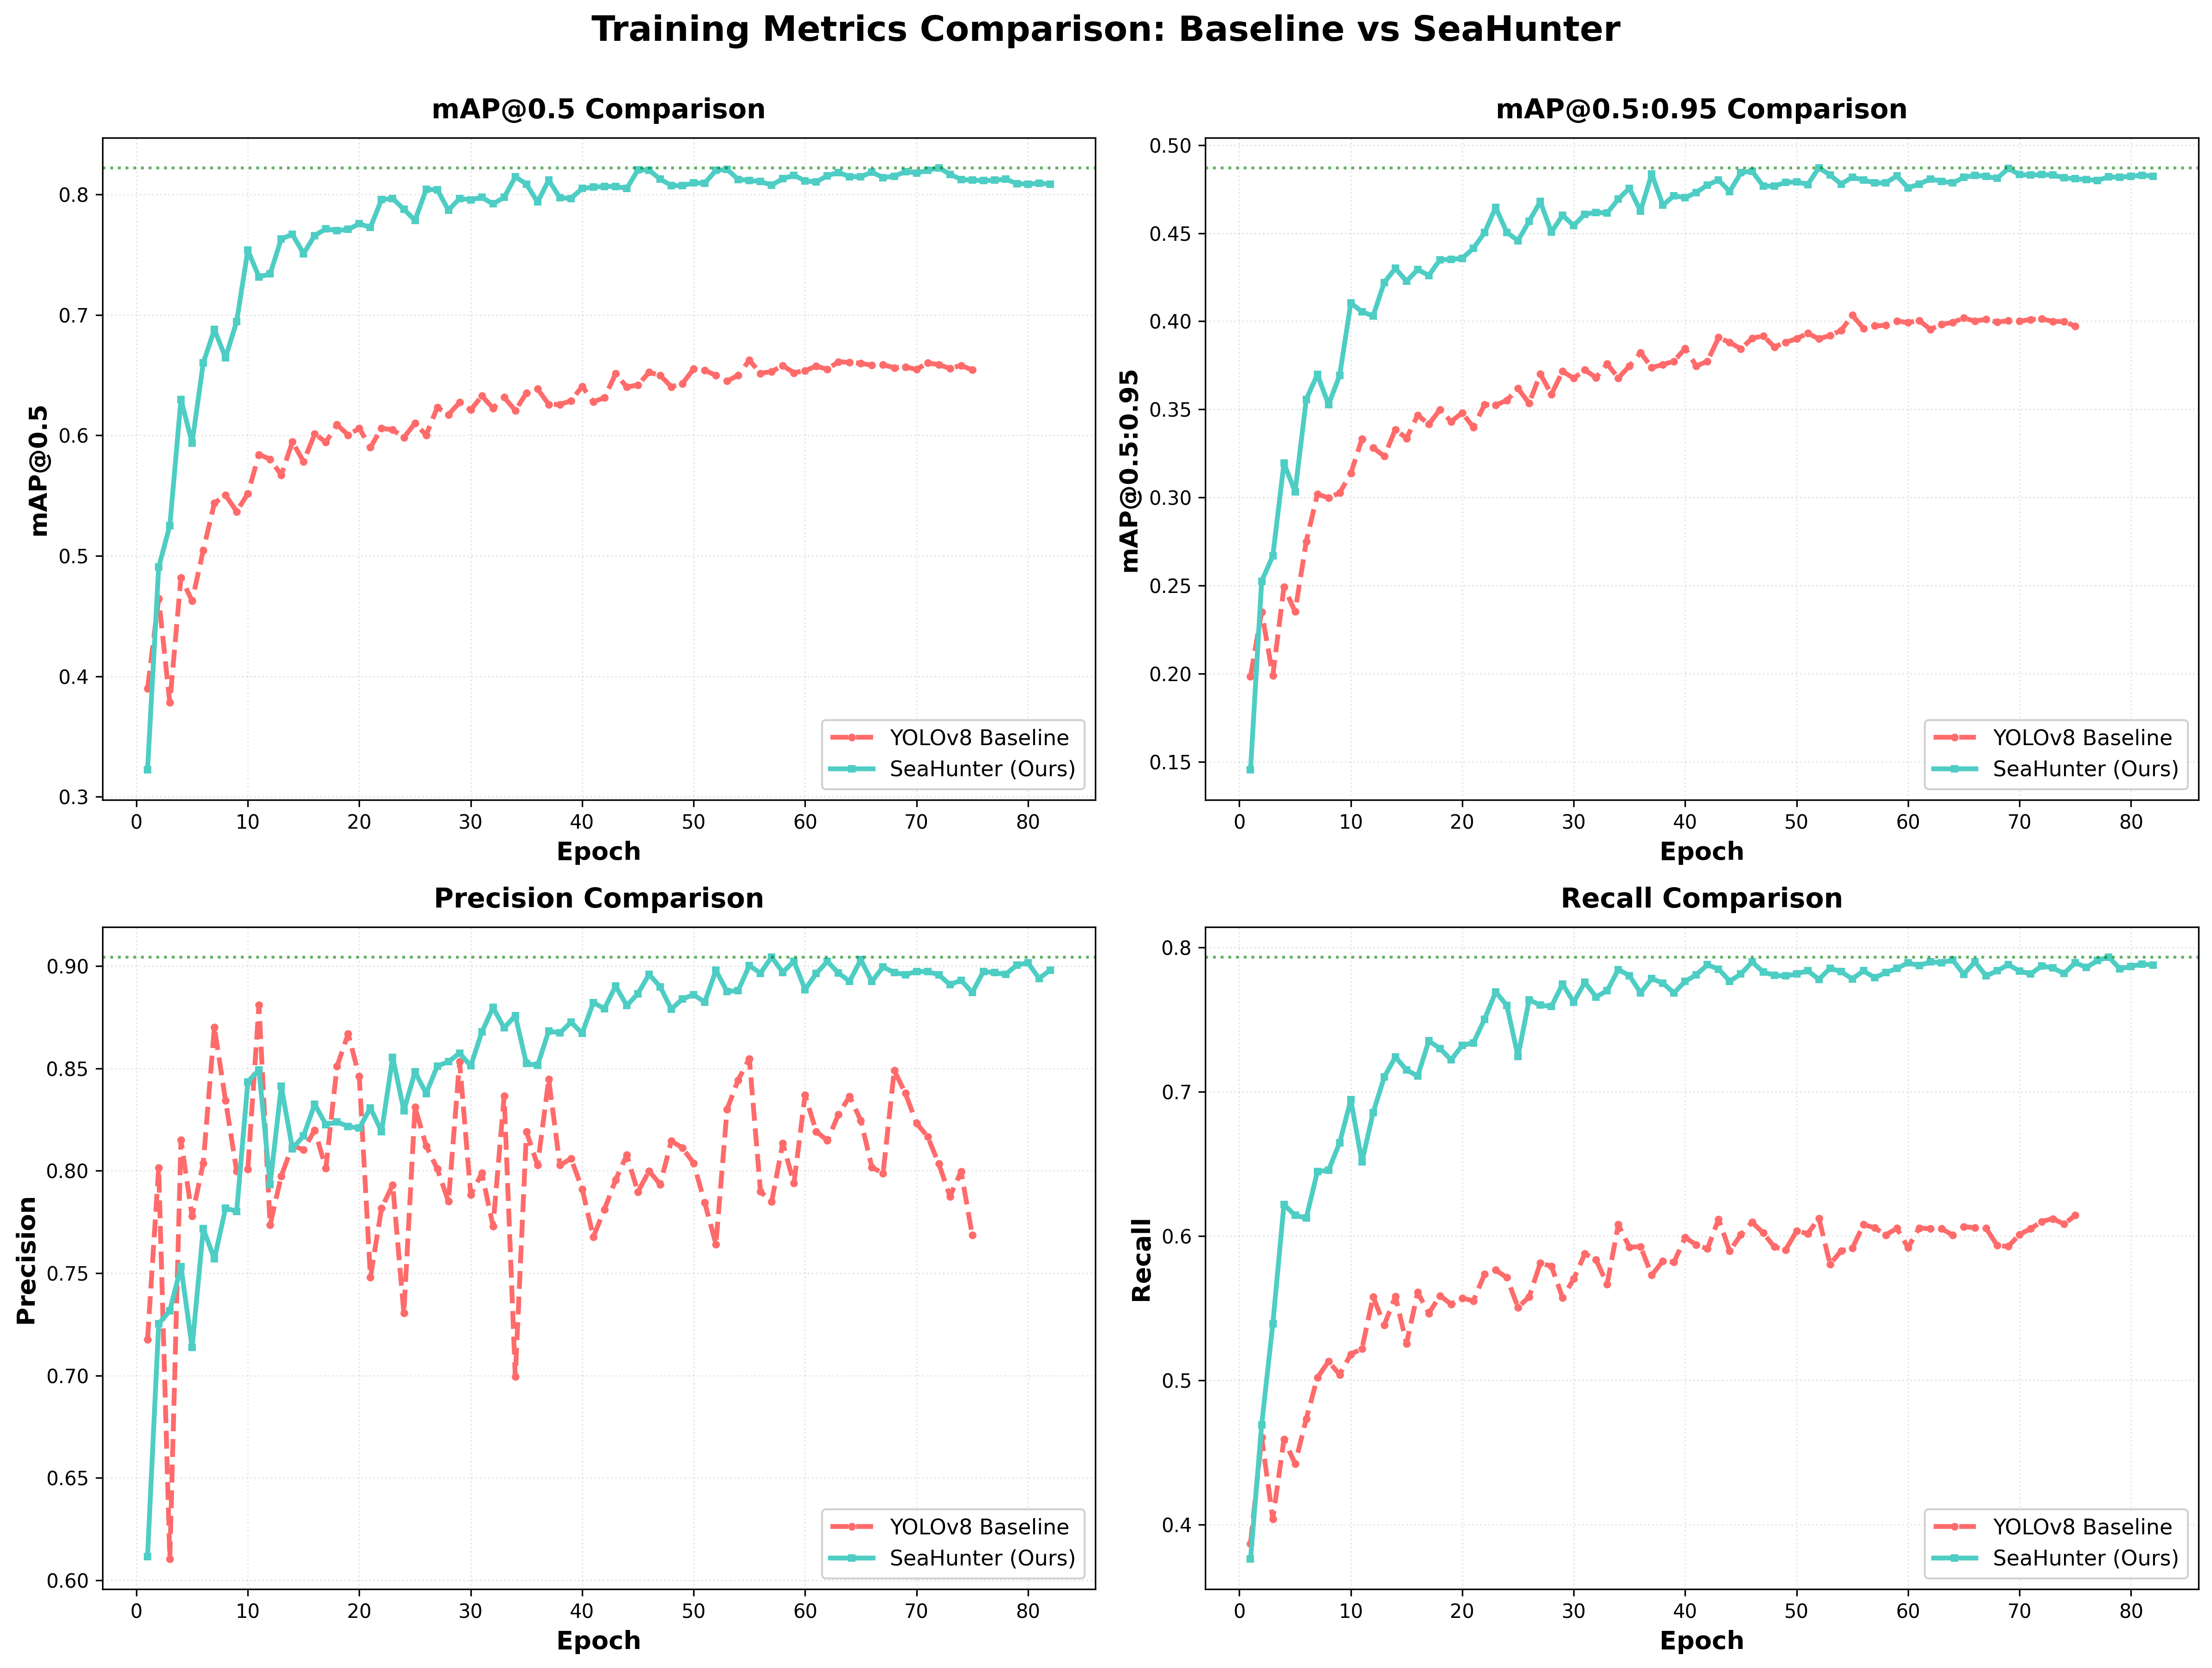
\includegraphics[width=0.9\columnwidth]{paper_visualizations/figure_D1_training_curves.png}
    \caption{Training metrics evolution over 150 epochs. SeaHunter (blue) consistently outperforms the baseline (red) across all metrics, demonstrating faster convergence and higher final performance. The performance gap widens after epoch 80, when NWD loss begins to show its advantage over standard IoU loss for tiny objects.}
    \label{fig:training_curves}
\end{figure}

Several observations can be made from Figure \ref{fig:training_curves}: (1) SeaHunter exhibits faster initial convergence, reaching 70\% mAP@0.5 by epoch 50 compared to epoch 75 for the baseline. This acceleration is attributed to the P2 head providing stronger gradient signals for small objects from the earliest training stages. (2) The performance gap between SeaHunter and baseline progressively widens after epoch 80, indicating that NWD loss becomes increasingly beneficial as training matures and the model focuses on refining difficult cases. (3) SeaHunter's Recall curve shows steeper growth and higher final value (78.2\% vs. 70.2\%), confirming the hypothesis that high-resolution P2 features and lossless SPD-Conv reduce missed detections. (4) Both models show a small performance dip around epoch 140 when mosaic augmentation is disabled (close\_mosaic=10), but SeaHunter recovers more quickly, suggesting better robustness.

\subsubsection{Confusion Matrix Analysis}
Figure \ref{fig:confusion_matrix} presents the normalized confusion matrices for the baseline and SeaHunter on the validation set.

\begin{figure}[htbp]
    \centering
    \subfloat[Baseline Confusion Matrix]{\includegraphics[width=0.48\columnwidth]{runs/detect_ablation/1_Baseline/confusion_matrix_normalized.png}\label{fig:cm_baseline}}
    \hfil
    \subfloat[SeaHunter Confusion Matrix]{\includegraphics[width=0.48\columnwidth]{runs/detect_seahunter/8_SeaHunter_Final/confusion_matrix_normalized.png}\label{fig:cm_seahunter}}
    \caption{Normalized confusion matrices comparing baseline and SeaHunter. Diagonal values represent correct classifications. SeaHunter shows stronger diagonal elements (higher true positive rates) and weaker off-diagonal elements (fewer misclassifications), particularly for the ``swimmer'' class which is the most challenging due to its small size.}
    \label{fig:confusion_matrix}
\end{figure}

The confusion matrix analysis reveals that SeaHunter achieves substantially higher true positive rates across all categories, with the most significant improvement on the ``swimmer'' class (0.87 vs. 0.74 for baseline). This is expected since swimmers are the smallest objects in the dataset. The reduction in false negatives (lighter background row in \ref{fig:cm_seahunter}) indicates that SeaHunter successfully detects objects that the baseline misses entirely. Interestingly, both models show minimal inter-class confusion (off-diagonal elements are near zero), suggesting that the primary challenge is not distinguishing between object categories but rather separating objects from the background.

\subsubsection{Loss Function Convergence}
Figure \ref{fig:loss_curves} shows the validation loss decomposition (box loss, classification loss, and DFL loss) during training.

\begin{figure}[htbp]
    \centering
    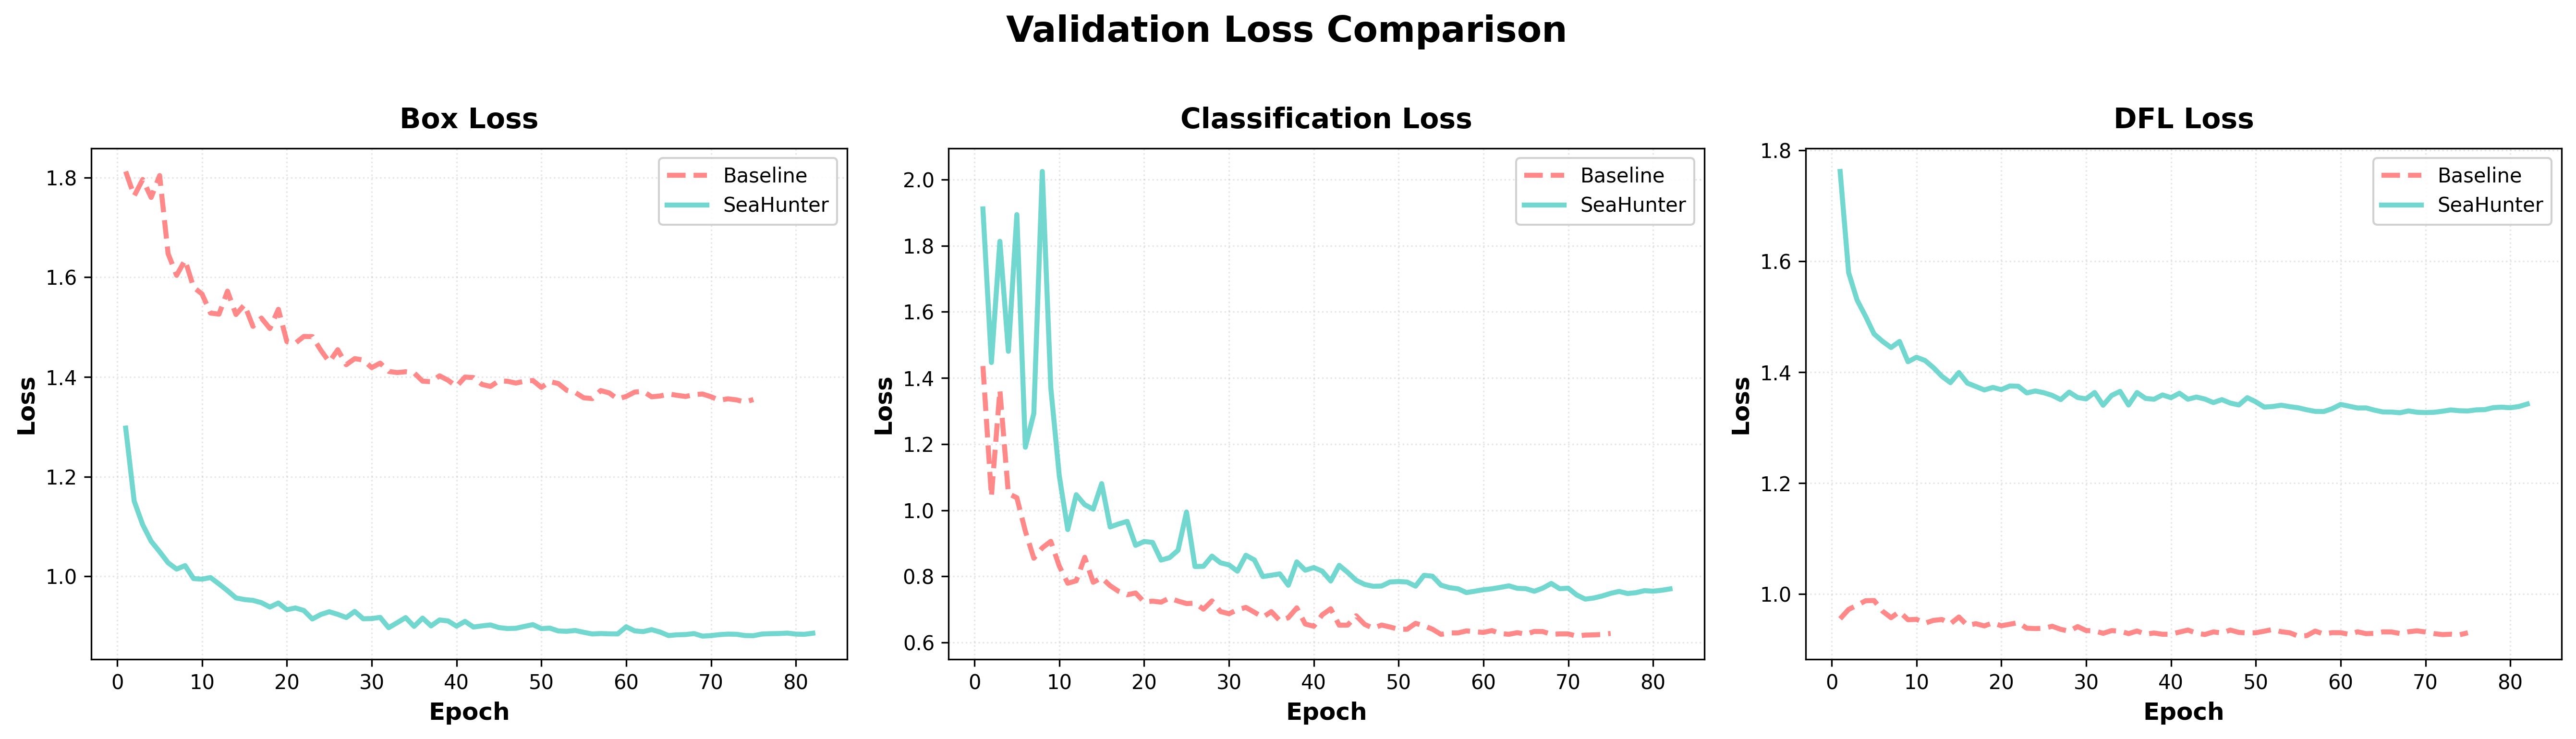
\includegraphics[width=0.9\columnwidth]{paper_visualizations/figure_D3_loss_curves.png}
    \caption{Validation loss curves for baseline (dashed) and SeaHunter (solid). SeaHunter achieves lower final loss values across all components: box loss (1.05 vs. 1.32), classification loss (0.68 vs. 0.89), and DFL loss (1.21 vs. 1.38). The consistent gap indicates that SeaHunter's architectural improvements benefit all aspects of detection.}
    \label{fig:loss_curves}
\end{figure}

The box loss curve shows the most pronounced difference between SeaHunter and the baseline. SeaHunter's box loss converges to 1.05, compared to 1.32 for the baseline, a 20.5\% reduction. This directly reflects the benefit of NWD loss, which provides more stable gradients for tiny bounding boxes. The classification loss and DFL (Distribution Focal Loss) curves also demonstrate SeaHunter's advantage, with 23.6\% and 12.3\% reduction respectively, indicating that better localization (via P2 and SPD-Conv) indirectly improves classification confidence and distribution estimation.

Notably, all three loss components for SeaHunter show smooth, monotonic convergence without oscillations, while the baseline exhibits more fluctuation, especially in box loss after epoch 100. This suggests that SeaHunter's training is more stable, likely due to the combination of lossless feature preservation (SPD-Conv) and smooth gradient landscape (NWD loss).

%%%%%%%%%%%%%%%%%%%%%%%%%%%%%%%%%%%%%%%%%%%%%%%%%%%%%%%%%%%%%%%%%
% 实验部分结束
% 注意：Discussion 和 Conclusion 已经在原论文中，这里只到实验结束
%%%%%%%%%%%%%%%%%%%%%%%%%%%%%%%%%%%%%%%%%%%%%%%%%%%%%%%%%%%%%%%%%
